\documentclass{llncs}

%\makeatletter
%\def\input@path{{../}}
%\makeatother
%

% Estos son los paquetes q ocupan todas las versiones del paper (normal y eprint)
\usepackage{setspace}
\usepackage{amsmath,amsfonts,amssymb,amstext}
\usepackage{mathtools}
\usepackage{latexsym,ifthen}
\usepackage{bbm,url}
\usepackage{float}
%\usepackage{bbold}
%\usepackage{amsthm}
\usepackage{bm}
\usepackage{xspace}
%\usepackage[pdftex,usenames,dvipsnames]{color}
\usepackage[usenames,dvipsnames]{color}
%\newtheorem{theorem}{Theoremh}
% \newtheorem{lemma}[theorem]{Lemma}
%\newtheorem{definition}{Definition}
%\newtheorem{example}{Example}
%\newtheorem{remark}{Remark}
%\usepackage{fullpage}
%\usepackage[margin=1.1in]{geometry}
\usepackage{tikz}
\usepackage{xspace}
\usetikzlibrary{arrows,chains,matrix,positioning,scopes,patterns}
\usepackage{authblk}
\usepackage[pdftex,pagebackref]{hyperref}
\usepackage{multirow}
\usepackage{wasysym}
%\usepackage{enumitem}
\usepackage[font=scriptsize]{caption}

% Temporal
\usepackage{soul}

%\usepackage[inline]{enumitem}
\usepackage{enumerate}

\newcommand{\err}{\mathsf{err}}

\newcommand{\cat}{|}
\newcommand{\dsum}{/}
\newcommand{\pdsum}[2]{\mathrm{diag}(#1,#2)}

\newcommand{\sblt}{\stackrel{s}{\bullet}}

\newcommand{\algSize}{normalsize} 
%\newcommand{\algSize}{footnotesize}
\newcommand{\sfleft}{{\mathsf{left}}}
\newcommand{\sfright}{{\mathsf{right}}}

\newcommand{\ps}{\Psi({\dist_k})}
\newcommand{\psws}{{\Psi(\overline{\dist}_k)}}
\newcommand{\sps}{{\Psi_{\mathsf{spl}}(\dist_k)}}
\newcommand{\Sps}{\Psi_{\mathsf{spl}}}
\newcommand{\spsws}{{\Psi_\mathsf{spl}(\overline{\dist}_k)}}
\newcommand{\Spsws}{\Psi_\mathsf{spl}}
\newcommand{\spsmas}{\Psi_{\sfsum}(\dist_k)}
\newcommand{\Spsmas}{\Psi_{\sfsum}}
\newcommand{\spswsmas}{\Psi_{\sfsum}(\overline{\dist}_k)}
\newcommand{\Spswsmas}{\Psi_{\sfsum}}
\newcommand{\spswscomm}{{\Psi_{\mathsf{com}}(\overline{\dist}_k)}}
\newcommand{\Spswscomm}{\Psi_{\mathsf{com}}}
\newcommand{\bbb}{\bar{b}}
\newcommand{\capprox}{\overset{c}{\approx}}

\newcommand{\latexDeMierdaEstupido}{]}

\newcommand{\Comm}{\mathsf{Comm}}
\newcommand{\Com}{\mathsf{Com}}
\newcommand{\vect}{\mathbf{vec}}

\newcommand{\lef}{{\mathtt{l}}}
\newcommand{\rig}{{\mathtt{r}}}
\newcommand{\stmnt}{\mathsf{stm}}
%Commitment keys

%Log Left Commitment Key
\newcommand{\llck}{\vecb{g}}
%Log Right Commitment Key
\newcommand{\lrck}{\vecb{h}}
%Left Commitment Key
\newcommand{\lck}{[{\llck}]_1}
%Right Commitment Key
\newcommand{\rck}{[{\lrck}]_2}
\newcommand{\rcks}{[{\lrck}]_1}

%Commitement keys matrices

%Log Left Commitment Keys
\newcommand{\Llck}{\matr{G}}
%Log Right Commitment Keys
\newcommand{\Lrck}{\matr{H}}
%Left Commitment Keys
\newcommand{\Lck}{[\Llck]_1}
%Right Commitment Keys
\newcommand{\Rck}{[{\Lrck}]_2}
\newcommand{\Rcks}{[{\Lrck}]_1}

%For quadratic info \lck\rck^\top
\newcommand{\Lqmatr}{\matr{C}}
\newcommand{\Qmatr}{{[\Lqmatr]_1}}
\newcommand{\Qspace}{\mathcal{C}}

% c_\Delta
\newcommand{\lccom}{\vecb{c}_\Delta}
\newcommand{\ccom}{\hvecb{c}_\Delta}

\newcommand{\pke}{\mathsf{PKE}}
\newcommand{\kem}{\mathsf{KEM}}
\newcommand{\prf}{\mathsf{PRF}}
\newcommand{\ev}{\mathsf{F}}
\newcommand{\KEM}{\mathsf{KEM}}
\newcommand{\gen}{\mathsf{Gen}}
\newcommand{\enc}{\mathsf{Enc}}
\newcommand{\Enc}{\mathsf{Enc}}
\newcommand{\dec}{\mathsf{Dec}}
\newcommand{\Dec}{\mathsf{Dec}}
\newcommand{\pk}{\mathit{pk}}
\newcommand{\sk}{\mathit{sk}}
\newcommand{\cdh}{\ensuremath{\mathsf{CDH}}}
\newcommand{\ddh}{\ensuremath{\mathsf{DDH}}}
\newcommand{\sxdh}{\ensuremath{\mathsf{SXDH}}}
\newcommand{\mddh}{\ensuremath{\mathsf{MDDH}}}
\newcommand{\mcdh}{\ensuremath{\mathsf{MCDH}}}
\newcommand{\fmdh}{\ensuremath{\mathsf{KerMDH}}}
\newcommand{\bddh}{\ensuremath{\mathsf{BDDH}}}
\newcommand{\mat}[1]{\ensuremath{#1\mbox{-}\mathsf{Mat}}}
\newcommand{\pddh}[1]{\ensuremath{#1\mbox{-}\mathsf{PDDH}}}
\newcommand{\mlddh}[1]{\ensuremath{#1\mbox{-}\mathsf{MLDDH}}}
\newcommand{\eddh}[1]{\ensuremath{#1\mbox{-}\mathsf{EDDH}}}
\newcommand{\casc}[1]{\ensuremath{#1\mbox{-}\mathsf{Casc}}}
\newcommand{\scasc}[1]{\ensuremath{#1\mbox{-}\mathsf{SCasc}}}
\newcommand{\lin}[1]{\ensuremath{#1\mbox{-}\mathsf{Lin}}}
\newcommand{\rlin}[1]{\ensuremath{#1\mbox{-}\mathsf{RLin}}}
\newcommand{\re}{\mathsf{RE}_\G}
\newcommand{\kcirc}[1]{\ensuremath{#1\mbox{-}\mathsf{Circ}}}
\newcommand{\escQE}{\gamma}
\newcommand{\EscQE}{\Gamma}


% M \in Z^{\la \times \lb}, N\in Z^{\la \times \lc}, \Lambda\in Z^{\ld\times \lb}
% x \in \Z_q^\la, b\in \Z_q^\lb, w\in\Z_q^\lc, \alpha\in \Z_q^\ld
\newcommand{\la}{{\ell_1}}
\newcommand{\lb}{{m}}
\newcommand{\lc}{{\ell_2}}
\newcommand{\ld}{{\ell_3}}


\newcommand{\LangMN}{{\Lang_{[\matr{M}]_1,[\matr{N}]_1,\matr{\Lambda},\grkb{\alpha}}}}



\newcommand{\skermdh}{\ensuremath{\mathsf{SKerMDH}}}
\newcommand{\kermdh}{\ensuremath{\mathsf{KerMDH}}}
\newcommand{\akermdh}{\ensuremath{\mathsf{aKerMDH}}}

\newcommand{\KG}{\mathsf{KeyGen}}
\newcommand{\GS}{{\mathsf{GS}}}

%HPS definitions
\newcommand{\univo}{universal$_1$\xspace}
\newcommand{\univt}{universal$_2$\xspace}
\newcommand{\distance}[2]{\Delta\left[#1 \,,\, #2\right]}
\newcommand{\entropic}{entropic\xspace}
\newcommand{\ciphertext}{{c}}
\def\params{\mathit{params}}
\newcommand{\structure}{\mathcal{S}}
\newcommand{\ciphersp}{\mathcal{C}}
\newcommand{\conssp}{\mathcal{V}}
\newcommand{\primeorder}{p}
\newcommand{\keysp}{\mathcal{K}}
\def\hps{\varfont{hps}}
\newcommand{\advBhps}{\calB}
\newcommand{\advBhpso}{\calB_{1}}
\newcommand{\advBhpst}{\calB_{2}}
\newcommand{\PK}{\mathcal{PK}}
\newcommand{\SK}{\mathcal{SK}}
\newcommand{\hash}{\mu}
\newcommand{\bigiota}{\mathcal{I}}
\newcommand{\var}[1]{{\mathsf{#1}}}
\newcommand{\vvar}[1]{{\mathbf{\var{#1}}}}
\newcommand{\varb}{\mathsf{b}}
\newcommand{\varx}{\mathsf{x}}
\newcommand{\vvarx}{\textbf{\textsf{x}}}
\newcommand{\vary}{\mathsf{y}}
\newcommand{\vvary}{\textbf{\textsf{y}}}
\newcommand{\varz}{\mathsf{z}}
\newcommand{\varX}{\mathsf{X}}
\newcommand{\varY}{\mathsf{Y}}
\newcommand{\varZ}{\mathsf{Z}}
\newcommand{\varvecx}{\vec{\varx}}
\newcommand{\varvecy}{\vec{\vary}}
\newcommand{\varvecz}{\vec{\varx}}
\newcommand{\hcx}{(\hat{x}_1,\ldots,\hat{x}_m)}
\newcommand{\matrB}{\matr{B}} 
\newcommand{\vecL}{(\hat{l}_1,\ldots,\hat{l}_n)}



% Las instancias de SPLHS se van a llamr \Phi
\newcommand{\SPLHSinst}{\Phi}
\newcommand{\SG}{\mathsf{SignGen}}
\newcommand{\SN}{\mathsf{Sign}}
\newcommand{\SD}{\mathsf{SignDerive}}
\newcommand{\SV}{\mathsf{Verify}}
\newcommand{\SP}{\ensuremath{\mathsf{SP}}}
\newcommand{\poly}{\mathsf{poly}}

%Comicmens a los eltos de la listas
\newcommand{\lcom}{\vecb{f}}
\newcommand{\Lcom}{\matr{F}}

%Definition
\newcommand{\MP}{\mathsf{MP}}
\newcommand{\GScom}{\mathsf{GS.Com_{\hvecb{U}}}}
\newcommand{\MPcomg}{\mathsf{MP.Com}_{\hmatr{G}}}
\newcommand{\MPcomh}{\mathsf{MP.Com}_{\hmatr{H}}}




% QA-NIZK for linear spaces
\newcommand{\ZKLinInst}{\mathsf{ZKLin}}
\newcommand{\ZKLinK}{\mathsf{ZKLin.K}_0}
\newcommand{\ZKLinKK}{\mathsf{ZKLin.K}_1}
\newcommand{\ZKLinCRS}{\mathsf{ZKLin.crs}}

\newcommand{\QANIZKsum}{{\spswsmas}}
\newcommand{\QANIZKcomms}{{\spswscomm}}
\newcommand{\QANIZKsym}{{\Psi_{\mathsf{sym}}}}

\newcommand{\nb}{{\overline{n}}}

\newcommand{\bb}{\overline{b}}
\newcommand{\bub}{{b(\overline{b}-1)}}
\newcommand{\tm}{\tilde{m}}

\newcommand{\rank}{\mathbf{rank}}
\newcommand{\HPSscheme}{\mathsf{HPS}}
%\newcommand{\THPSscheme}{\schemefont{HPS_t}}
% \newcommand{\THPSscheme}{\mathsf{HPS^{td}}}
% \newcommand{\HHPSscheme}{\mathsf{HPS}_2}
\newcommand{\HPSsys}{\mathsf{Param}}
\newcommand{\HPSpub}{\mathsf{Pub}}
\newcommand{\HPSpriv}{\mathsf{Priv}}
\newcommand{\HPSdec}{\mathsf{Decide}}
\newcommand{\eval}{\Lambda}
%\newcommand{\hpscu}{{\notionfont{cu}_2}}
%\newcommand{\ExpHPScu}[2]{\Exp^{\hpscu}_{#1,#2}}
%\newcommand{\AdvHPScu}[2]{\Adv^{\hpscu}_{#1,#2}}
%\newcommand{\hpscub}{{\notionfont{\hpscu\mbox{-}b}}}
%\newcommand{\hpscuz}{{\notionfont{\hpscu\mbox{-}0}}}
%\newcommand{\hpscuo}{{\notionfont{\hpscu\mbox{-}1}}}
%\newcommand{\ExpHPScub}[2]{\Exp^{\hpscub}_{#1,#2}}
%\newcommand{\ExpHPScuo}[2]{\Exp^{\hpscuo}_{#1,#2}}
%\newcommand{\ExpHPScuz}[2]{\Exp^{\hpscuz}_{#1,#2}}
% \newcommand{\pcol}{\delta}
\newcommand{\prcol}{\delta}
\newcommand{\trapdoor}{\omega}
\newcommand{\witness}{r}
\newcommand{\algD}{\mathsf{D}}
\newcommand{\algK}{\mathsf{K}}
\newcommand{\algG}{\mathsf{G}}
\newcommand{\algP}{\mathsf{P}}
\newcommand{\algV}{\mathsf{V}}
\newcommand{\algS}{\mathsf{S}}
\newcommand{\algF}{\mathsf{F}}
\newcommand{\algVrfy}{\mathsf{Vrfy}}

\newcommand{\R}{\mathcal{R}}
\newcommand{\M}{\mathcal{M}}
\newcommand{\dist}{\mathcal{D}}
\newcommand{\distw}{\mathcal{W}}
\newcommand{\distk}{\mathcal{K}}
\newcommand{\distlin}{\mathcal{L}}
\newcommand{\distrlin}{\mathcal{RL}}
\newcommand{\distc}{\mathcal{C}}
\newcommand{\distsc}{\mathcal{SC}}
\newcommand{\distcirc}{\mathcal{CI}}
\newcommand{\distu}{\mathcal{U}}
\newcommand{\distp}{\mathcal{P}}
\newcommand{\distink}{\dist_k^{m,i}}
\newcommand{\distjnk}{\dist_1^{m,i}}

\newcommand{\distinmk}{\dist_k^{mn,i}}
\newcommand{\distzeronmk}{\dist_k^{mn,0}}
\newcommand{\distzeronk}{\dist_k^{m,0}}
\newcommand{\distlininone}{\distlin_1^{m,i}}
\newcommand{\distlinisnone}{\distlin_1^{m,i^*}}
\newcommand{\distlinizeroone}{\distlin_1^{m,0}}
\newcommand{\distlinjsnzero}{\distlin_1^{n,j^*}}
\newcommand{\block}[1]{
  \underbrace{\begin{matrix}1 & \cdots & 1\end{matrix}}_{#1}
}
%\newcommand{\gets}{\leftarrow}
\newcommand{\Z}{\mathbb{Z}}
\newcommand{\N}{\mathbb{N}}
\newcommand{\G}{\mathsf{Gen}}
\newcommand{\advD}{\mathsf{D}}
\newcommand{\advA}{\mathsf{A}}
\newcommand{\advB}{\mathsf{B}}
\newcommand{\adv}{\mathbf{Adv}}
\newcommand{\group}{{gk}}
\newcommand{\gk}{\group}
\newcommand{\pgroup}{\mathcal{PG}}
\newcommand{\mgroup}[1]{\mathcal{MG}_{#1}}
\newcommand{\ggen}{\mathsf{Gen}}
\newcommand{\pggen}{\mathsf{PGen}}
\newcommand{\mggen}[1]{\mathsf{MGen}_{#1}}
\newcommand{\heading}[1]{\smallskip\noindent{\sc{#1}}}
\newcommand{\vecb}[1]{{\boldsymbol{#1}}}
\newcommand{\vecbt}[1]{\vec{#1}^{\ \top}}
\newcommand{\uvecb}[1]{{\vect({\vecb{#1}})}}
\newcommand{\tvecb}[1]{{\tilde{\vecb{#1}}}}
\newcommand{\tgrkb}[1]{\tilde{\grkb{#1}}}
\newcommand{\ovecb}[1]{{\overline{\vecb{#1}}}}
\newcommand{\Pt}{\mathcal{P}}
\newcommand{\Opt}{\mathcal{O}}
\newcommand{\pt}[1]{\mathcal{#1}}
\newcommand{\stbl}{\ \tilde \bullet \ }
\newcommand{\bilgroup}{\mathcal{PG}}
\newcommand{\matr}[1]{\mathbf{{#1}}}
\newcommand{\vecw}{\vecb{w}}
\newcommand{\vecr}{\vecb{r}}
\newcommand{\vecz}{\vecb{z}}
\newcommand{\vecy}{\vecb{y}}
\newcommand{\vecx}{\vecb{x}}
\newcommand{\veca}{\vecb{a}}
\newcommand{\matrA}{\matr{A}}
\newcommand{\hmatrA}{\hmatr{A}}
\newcommand{\cmatrA}{\cmatr{A}}
\newcommand{\smallpmatrix}[1]{\left(\begin{smallmatrix}#1\end{smallmatrix}\right)}
\newcommand{\pmatri}[1]{\left(\begin{matrix}#1\end{matrix}\right)}
\newcommand{\bmatri}[1]{\left[\begin{matrix}#1\end{matrix}\right]}
\newcommand{\matri}[1]{{\begin{matrix}#1\end{matrix}}}
\newcommand{\smatri}[1]{{\begin{smallmatrix}#1\end{smallmatrix}}}
\newcommand{\sfsplit}{\mathsf{spl}}
\newcommand{\bulletsp}{ \bullet }
\newcommand{\newf}{\widehat{f}}
\newcommand{\newF}{\widehat{F}}
\newcommand{\com}{\mathsf{com}}
\newcommand{\eq}{\mathsf{eq}}
\newcommand{\eqd}{\equiv}
\newcommand{\negl}{\mathsf{negl}}
\newcommand{\A}{\mathcal{A}}
\newcommand{\GG}{\mathbb{G}}
\newcommand{\ZZ}{\mathbb{Z}}
\newcommand{\Gr}{\ensuremath{\mathbb{G}_1}}
\newcommand{\Hr}{\ensuremath{\mathbb{G}_2}}
\newcommand{\T}{\ensuremath{\mathbb{T}}}
\newcommand{\SSDP}{\ensuremath{\mathsf{SSDP}}}
\newcommand{\PermP}{\ensuremath{\mathsf{PermP}}}
\newcommand{\PP}{\ensuremath{\mathsf{PP^*}}}
\newcommand{\bmatr}[1]{\left[\matr{#1}\right]}
\newcommand{\hmatr}[1]{{\hat{\matr{#1}}}}
\newcommand{\cmatr}[1]{\check{\matr{#1}}}
\newcommand{\bvecb}[1]{\left[\vecb{#1}\right]}
\newcommand{\hvecb}[1]{{\hat{\vecb{#1}}}}
\newcommand{\cvecb}[1]{\check{\vecb{#1}}}
\newcommand{\bits}{\{0,1\}}
\newcommand{\rmIm}{\mathbf{Im}}
\newcommand{\sfGame}{\mathsf{Game}}
\newcommand{\sfReal}{\mathsf{Real}}
\newcommand{\grkb}[1]{{\boldsymbol #1}}
\newcommand{\ugrkb}[1]{{\underline{\grkb{#1}}}}
\newcommand{\hgrkb}[1]{\hat{\grkb{#1}}}
\newcommand{\cgrkb}[1]{\check{\grkb{#1}}}
\newcommand{\SDP}{\ensuremath{\mathsf{SDP}}}
\newcommand{\Span}{\mathbf{Span}}
\newcommand{\Group}{G}
\newcommand{\Forger}{\mathsf{F}}
\newcommand{\advSound}{\mathsf{P}^*}
\newcommand{\Lang}{\mathcal{L}}
\newcommand{\crs}{\mathsf{crs}}
\newcommand{\sfproof}{\mathsf{proof}}
\newcommand{\sfbits}{\mathsf{bits}}
\newcommand{\sfbitsn}{{\mathsf{bits},n}}
\newcommand{\sflin}{\mathsf{lin}}
\newcommand{\sfcom}{\mathsf{com}}
\newcommand{\sfbin}{\mathsf{bin}}
\newcommand{\sfset}{\mathsf{set}}
\newcommand{\sfsum}{\mathsf{sum}}
\newcommand{\rp}{{\mathsf{range}\mbox{-}\mathsf{proof}}}
\newcommand{\ovG}{\overline{\matr{G}}}
\newcommand{\ovc}{\overline{\vecb{c}}}
\newcommand{\ovb}{\overline{\vecb{b}}}

\newcommand{\dmatrix}[1]{\begin{pamtrix}#1 & \cdots & \vecb{0}\\\vdots & \ddots & \vdots\\\vecb{0}& \ldots & #1\end{pmatrix}}
\newcommand{\sdmatrix}[1]{\smallpmatrix{#1 & \cdots & \vecb{0}\\\vdots & \ddots & \vdots\\\vecb{0}& \ldots & #1}}


%weas q hay que hacer pa q no webee el latex
\newsavebox{\smlmat}% Box to store smallmatrix content
\newsavebox{\smat}
\savebox{\smlmat}{$\left(\begin{smallmatrix}
\matr{G}_1 & \ldots & \vecb{0}   & \vecb{g}_{n+1} & \ldots & \vecb{0}\\
\vdots     & \ddots & \vdots     & \vdots         & \ddots & \vdots\\
\vecb{0}   & \ldots & \matr{G}_1 & \vecb{0}       & \ldots & \vecb{g}_{n+1}
\end{smallmatrix}\right)$}

\savebox{\smat}{$\left(\begin{matrix}
s_1 & \ldots & s_n\\
0   & \ldots & 0
\end{matrix}\right)$}






\newcommand{\sG}{|\GG_1|}
\newcommand{\sH}{|\GG_2|}
\newcommand{\s}{(\sG+\sH)}

\newcommand{\vu}{\hat{\vecb{u}}}
%\newcommand{\vv}{\check{\vecb{v}}}
\newcommand{\vc}{\hat{\vecb{c}}}
\newcommand{\vd}{\check{\vecb{d}}}
\newcommand{\zip}{\mathbf{zip}}

\newcommand{\indexSet}[2]{\mathcal{I}_{#1,#2}}
\newcommand{\SignaturesSet}{\mathcal{S}}
\newcommand{\KGen}{\mathsf{KGen}}
\newcommand{\Sign}{\mathsf{Sign}}
\newcommand{\Ver}{\mathsf{Ver}}

\newcommand{\bit}{\mathsf{bit}}
\newcommand{\sfts}{\mathsf{ts}}

%El-Gamal keys
\newcommand{\egpk}{\hat{x}}
\newcommand{\egsk}{x}
\newcommand{\egvpk}{\hvecb{k}}
\newcommand{\egvsk}{\vecb{k}}

%The set of permutation matrices
\newcommand{\matrPerms}{\mathcal{S}}
%The set of permutations
\newcommand{\Perms}{S}

\newcommand{\duda}[1]{{\iffalse\color{red}#1\fi}}

\newcommand{\cambio}[2]{{\iffalse\color{blue}Ahora: \fi#1}{\iffalse\color{red}(Antes: #2)\fi}}

\newenvironment{code}
   {\begin{tabbing}
   \hspace{4mm} \= \hspace{4mm} \= \hspace{4mm} \= \hspace{4mm} \= \hspace{4mm} \= \kill \\
   }
   {\end{tabbing}}

%\newcommand{\authnote}[2]{\medskip \noindent {\bf #1 says:} #2}
\newcommand{\authnote}[2]{\medskip \noindent {\bf #1 says:} {\textcolor{blue}{#2}}}

%\newtheorem{corollary}{Corollary}

\newtheorem{fact}{Fact}
\newtheorem{observation}{Observation}

\newcommand{\Am}{A}
\newcommand{\vX}{\ensuremath{\hat{\vecb{x}}}}
\newcommand{\VX}{\ensuremath{\hat{\vecb{v}}}}
\newcommand{\WX}{\ensuremath{\hat{\vecb{w}}}}
\newcommand{\VY}{\ensuremath{\check{\vecb{v}}}}
\newcommand{\WY}{\ensuremath{\check{\vecb{w}}}}
\newcommand{\vy}{\ensuremath{\vecb{y}}}
\newcommand{\vY}{\ensuremath{\check{\vecb{y}}}}
\newcommand{\vx}{\ensuremath{\vecb{x}}}


\newcommand{\U}{\ensuremath{\vecb{u}}}
\newcommand{\V}{\ensuremath{\vecb{v}}}
\newcommand{\vr}{\ensuremath{\vecb{r}}}
\newcommand{\vs}{\ensuremath{\vecb{s}}}
\newcommand{\vt}{\ensuremath{\vecb{t}}}


\newcommand{\ux}{\ensuremath{\hat{\vecb{u}}}}
\newcommand{\uy}{\ensuremath{\check{\vecb{u}}}}

\newcommand{\minitbl}[2]{\begin{tabular}{l}{#1}\\{#2}\end{tabular}}

\newcommand{\ef}{\iffalse}
%
%\makeatletter
%\newcommand*{\inlineequation}[2][]{%
%  \begingroup
%    % Put \refstepcounter at the beginning, because
%    % package `hyperref' sets the anchor here.
%    \refstepcounter{equation}%
%    \ifx\\#1\\%
%    \else
%      \label{#1}%
%    \fi
%    % prevent line breaks inside equation
%    \relpenalty=10000 %
%    \binoppenalty=10000 %
%    \ensuremath{%
%      % \displaystyle % larger fractions, ...
%      #2%
%    }%
%    ~\@eqnnum
%  \endgroup
%}
%\makeatother
%
%\makeatletter
%\renewcommand*{\@opargbegintheorem}[3]{\trivlist
%  \item[\hskip \labelsep{\bfseries #1\ #2}] \textbf{(#3)}\ \itshape}
%\makeatother


\pagestyle{plain}

\author{Alonso Gonz\'alez}
\institute
{
	Ecole Normale Sup´\'erieure de Lyon, Laboratoire LIP (France)\\
	\email{alonso.gonzalez@ens-lyon.fr}
}

\title{A Ring Signature of size $\Theta(\sqrt[3]{n})$ without Random Oracles}
\begin{document}
	
\maketitle
\begin{abstract}
    % !TEX root = ./main-ring-signature.tex

Ring signatures, introduced by Rivest, Shamir and Tauman (ASIACRYPT 2001), allow to sign a message on behalf of a set of users while guaranteeing authenticity and anonymity. In terms of efficiency, one of the shortest ring signatures are of size $\Theta(\log n)$, where $n$ is the number of users, and are due to Groth and Kohlweiss (EUROCRYPT 2015) and Libert et al.~(EUROCRYPT 2016). An even shorter ring signature, of size independendent from the number of users, was recently proposed by Malavolta and  Schr\"oder (ASIACRYPT 2017).
However, the former schemes are both proven secure in the random oracle model while the later requires non-falsifiable assumptions. Under more standard and plausible assumptions, the most efficient construction remains the one of Chandran et al.~(ICALP 2007) with a signature of size $\Theta(\sqrt{n})$ and no improvements in the signature size have been made within a decade.

In this work we construct an asymptotically shorter ring signature without random oracles or non-falsifiable assumptions. Our construction uses bilinear groups and we prove its security under the permutation pairing assumption, introduced by Groth and Lu (ASIACRYPT 2007).
 Each signature comprises $\Theta(\sqrt[3]{n})$ group elements, signing a message requires computing $\Theta(\sqrt[3]{n})$ exponentiations, and verifying a signature requires $\Theta(n^{2/3})$ pairing operations. To the best of our knowledge, this is the first ring signature with subquadraic signatures and sublinear verification complexity in this setting.

\end{abstract} 

\section{Introduction}

    Ring signatures, introduced by Rivest, Shamir and Tauman, \cite{AC:RivShaTau01}, allow to anonymously sign a message on behalf of a ring of users $P_1,\ldots,P_n$, only if the signer belongs to that ring. Although there are other cryptographic schemes that provide similar guarantees (e.g.~group signatures \cite{EC:ChaVan91}), ring signatures are not coordinated: each user generates secret/public keys on his own -- i.e.~no central authorities -- and might sign on behalf of a ring without the approval or assistance of the other members.

While the more efficient constructions have signature size logarithmic in the size of the ring \cite{EC:GroKoh15,EC:LLNW16}, all of them rely on the {random oracle model}.
Without random oracles all constructions have signatures of size linear in the size of the ring, being the sole exception the $\Theta(\sqrt{n})$ ring signature of Chandran et al.~\cite{ICALP:ChaGroSah07}. 
We remark that no asymptotic improvements to Chandran et al.'s construction have been made since their introduction (only improvements in the constants by R\`afols \cite{TCC:Rafols15} and by Gonz\'alez et al.~\cite{AC:GonHevRaf15}). Although some previous works claim to construct signatures of constant \cite{ACISP:BosDasRan15} or logarithmic \cite{IET:GriSusPla16} size, they are either in a weaker security model or we can identify a flaw in the construction (see Section \ref{sec:rs-flawed}). 

In this work we present the first ring signature (without random oracles) whose signature size is asymptotically smaller than Chandran et al.'s. Our ring signature consists of $\Theta(\sqrt[3]{n})$ group elements, computing a signature requires $\Theta(\sqrt[3]{n})$ exponentiations, and verifying a signature requires $\Theta(n^{2/3})$ pairings.

The security of our construction relies on a security assumption -- the {permutation pairing assumption} -- introduced by Groth and Lu \cite{AC:GroLu07} in an unrelated setting: proofs of correctness of a shuffle. While the assumption is ``non-standard'', in the sense that is not a ``DDH like'' assumption, it is a falsifiable assumption and it was proven hard in generic symmetric groups by Groth and Lu. For simplicity, we work on symmetric groups ($\GG_1=\GG_2$) but our techniques can be easily extended to asymmetric groups as we show in Appendix \ref{sec:aPPA}.

Our ring signature outperforms Chandran et al.'s in terms signature size for any $n > 246$, in terms of signature generation time for any $n>205$, and in terms of verifier efficiency for any $n>170$. However, this analysis should be taken with care, since Chandran et al.'s signature is proven secure under the decisional linear (DLin) assumption while ours is proven secure under the permutation pairing assumption. Therefore, it could be the case that our scheme would be as secure as Chandran et al.'s at higher values of the security parameter. In Table \ref{table:eff} we provide a comparison between our scheme and Chandran et al.'s.

% !TEX root = ../main-ring-signature.tex

\begin{table}[h]
\begin{center}
\begin{minipage}{\textwidth}
\begin{center}
%\begin{scriptsize}
\begin{tabular}{l|l|l}
%\hline
                                           & Chandran et al.~\cite{ICALP:ChaGroSah07} & This work \\
\hline%\hline
\rule{0pt}{2.5ex}CRS size  $\GG_1/\GG_2$              & 4/4                                      & $4/4$       \\
\rule{0pt}{2.5ex}Verification key size $\GG_1/\GG_2$    & $1/0$                                       & $2/5$       \\
\rule{0pt}{2.5ex}Signature size      $\GG_1/\GG_2$      & $12\sqrt{n}+10/15\sqrt{n}+8$                        & $24\sqrt[3]{n} + 36/34\sqrt[3]{n} + 24$\\
\rule{0pt}{2.5ex}Signature generation time & $37\sqrt{n}+23$                        & $80\sqrt[3]{n}+71$\\
\rule{0pt}{2.5ex}Verification time         & $2n + 60\sqrt{n}+38$                & $8n^{2/3} + 162\sqrt[3]{n} + 118$\\
%\hline 
\end{tabular}
%\end{scriptsize}
\end{center}
\caption{Comparison of Chandran et al.'s ring signature and ours for a ring of size $n$. 'Signature generation time' is measured in number of exponentiations, 'Verification time' is measured in number of pairings, and all other rows are measured in number of group elements.\label{table:eff}}
\end{minipage}
\end{center}
\end{table}

%
%\begin{figure}[!t]
%	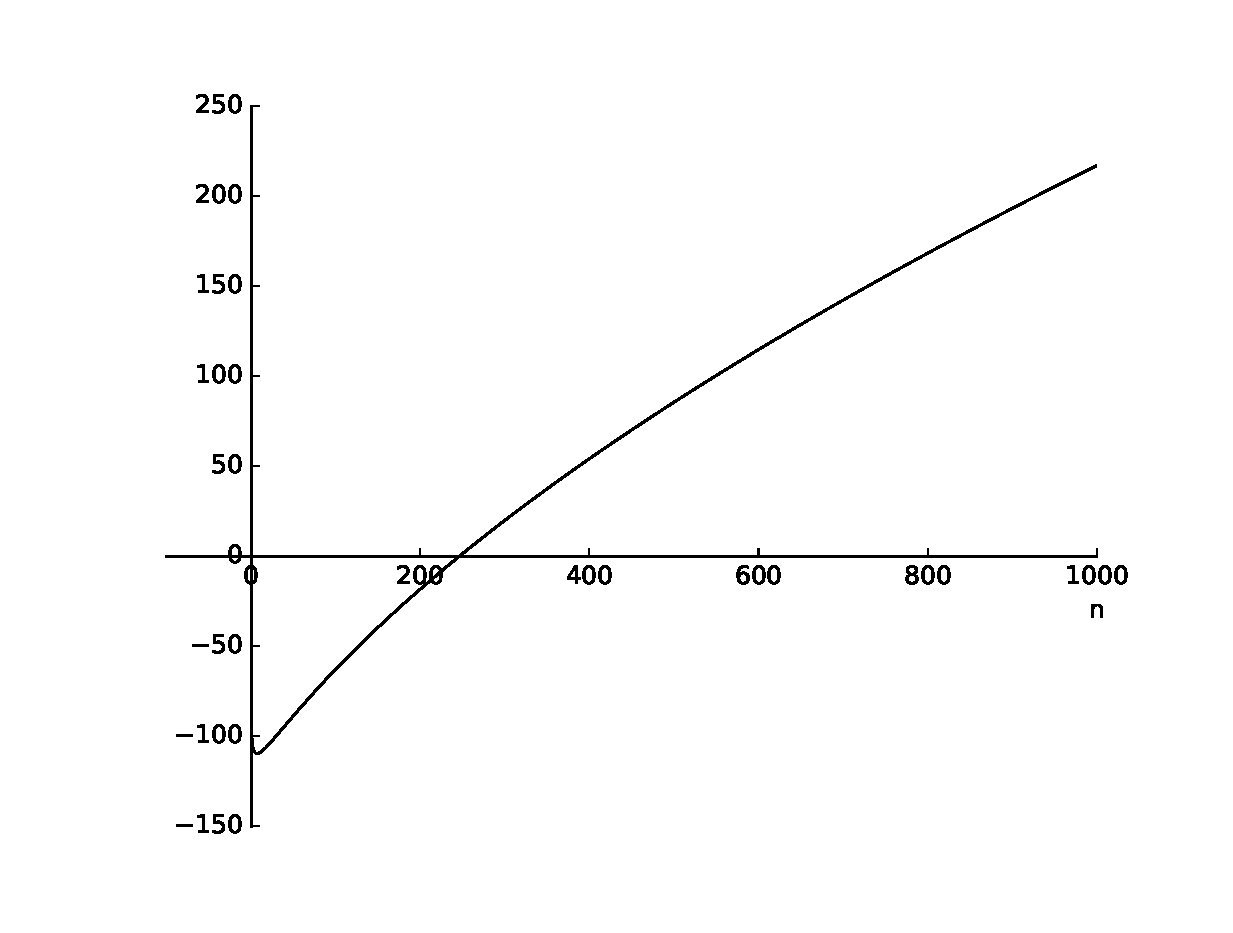
\includegraphics[scale=.25]{intro/sign_size}
%	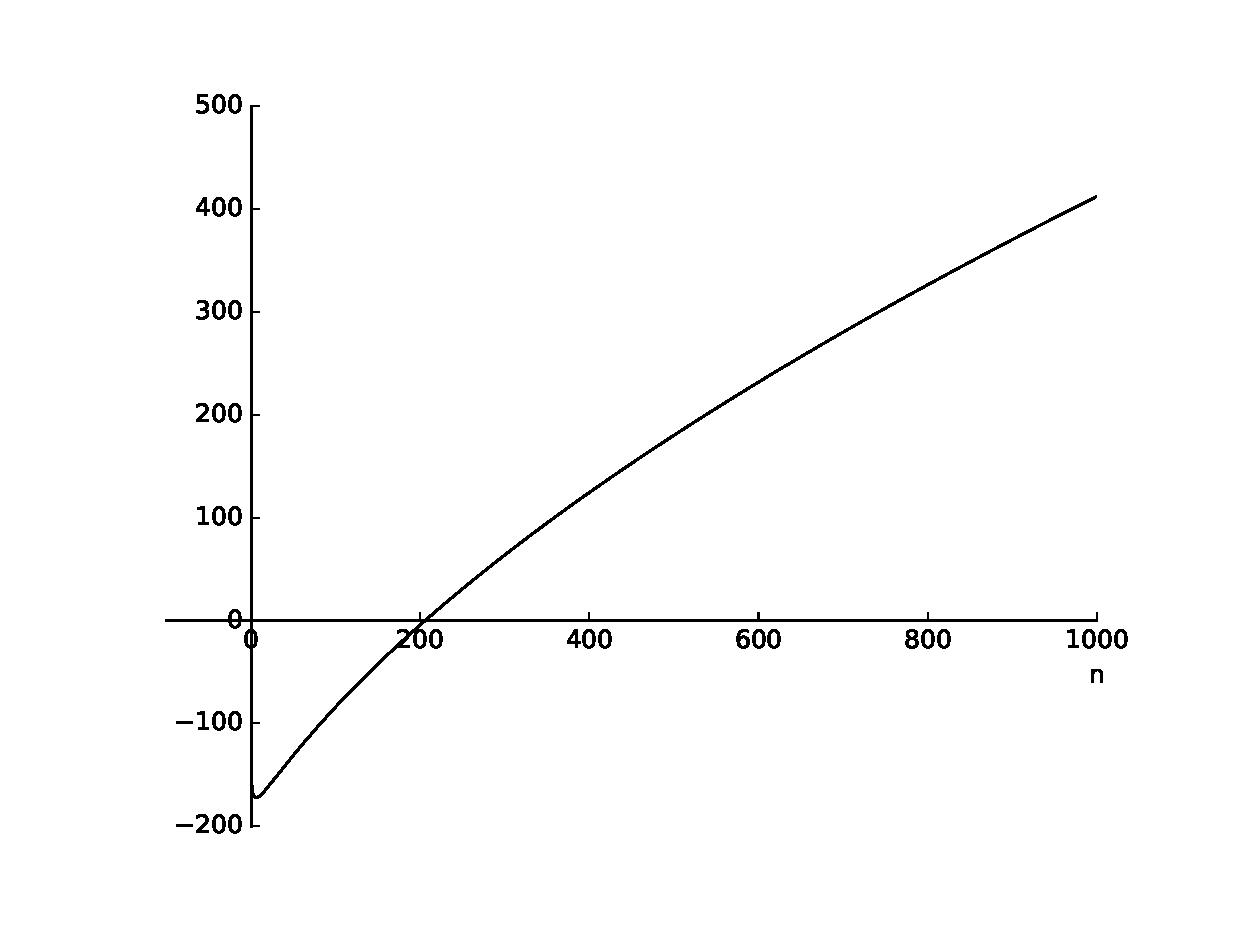
\includegraphics[scale=.25]{intro/sign_time}
%	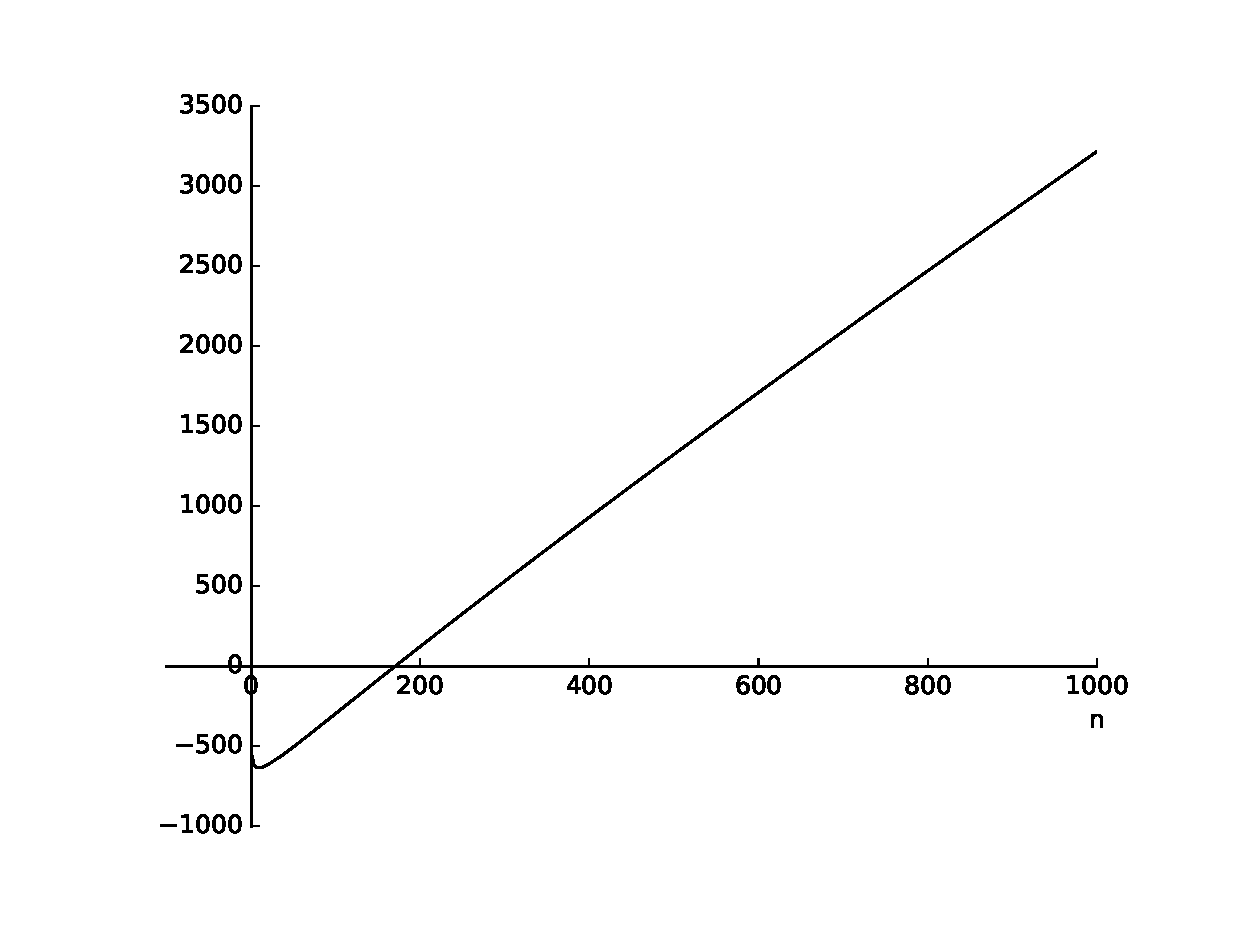
\includegraphics[scale=.25]{intro/ver_time}
%\end{figure} 

   \subsection{Technical Overview} \label{sec:tech-overview}

	% !TEX root = ../main-ring-signature.tex

To give a more clear understanding our contributions, it will be illustrative to see what is the main difficulty when constructing a ring signature on bilinear groups. Most schemes have followed the following approach. Given a ring of users defined by the set of their public keys and a message: a) sign the message, b) prove in zero-knowledge knowledge of a signature which can be verified using some committed/randomized verification key, and then c) prove in zero-knowledge that this verification key belongs to the set of public keys in the ring.  The most expensive part is c) and is sometimes called a \emph{set-membership proof}.

In the case of a ring signature, a set-membership has the following additional property: \emph{all the verification keys forming the ring are honestly generated}. 
Indeed, since the set-membership proof is only used to guarantee unforgeability, it makes no sense to guarantee unforgeability when members of the ring are controlled by the adversary.
It turns out that all the schemes we are aware of, in particular Chandran et al.'s, obviate this property, meaning that their set membership proofs are for adversarially chosen verification keys.
We ask the following natural question.
\begin{displayquote}
Can we construct more efficient set membership proofs (without random oracles or non-falsifiable assumptions) when verification keys are sampled from a known distribution?
\end{displayquote}
We answer this question in the affirmative and we construct a $\Theta(\sqrt[3]{n})$ set membership proof when the verification keys are honestly sampled. In contrast, Chandran et al.'s proof is of size $\Theta(\sqrt{n})$ but it makes no assumption on the verification keys distribution.

Our main technical tool is a structure preserving --- i.e.~compatible with Groth-Sahai proofs --- hash function with \emph{always second-preimage resistance} (aSec in the terminology of Rogaway and Shrimpton \cite{FSE:RogShr04}). That is, given $A$ in the domain of $h$, is hard to find $A'\neq A$ such that $h(A')=h(A)$ {\bf whenever $A$ is randomly sampled from the domain}.
Our function $h$ takes as input $A$, a set of verification keys (in fact, a fragment of each verification key), and returns a constant size digest which is simply $h(A)= \sum_{\vecb{a} \in A} \vecb{a}$. Thereby, whenever $h$ is applied to a set of honestly sampled verification keys, $A$ is indeed random and hence is infeasible to compute a second preimage.

\subsubsection{High level description}
We construct a set membership proof where a prover wants to convince a verifier that some commitment $c$ opens to $\vecb{a}$ and $\vecb{a}\in\{\vecb{a}_1,\ldots,\vecb{a}_n\}$. To do so, we arrange the $n$ elements of the ring into $n^{2/3}$ blocks of size $m=\sqrt[3]{n}$. We coin the following notation: for a ring $\{\vecb{a}_i:1\leq i \leq n\}$ define $\vecb{a}_{\mu,\nu}:=\vecb{a}_{(\mu-1)m+\nu}$, where  $1\leq\mu\leq n^{2/3},1\leq \nu\leq m$.  Let
\begin{align*}
& A_1 := \{\vecb{a}_{1,1},\ldots,\vecb{a}_{1,m}\},\ldots, A_{n^{2/3}} := \{\vecb{a}_{n^{2/3},1},\ldots,\vecb{a}_{n^{2/3},m}\},\,
H:=\{h(A_1),\ldots,\allowbreak h(A_{n^{2/3}})\}.
\end{align*}

We use Chandran et al.'s underlying set membership proof of size $\Theta(\sqrt{n})$ to prove knowledge of some $h(A_\mu)\in H$. Since $|H|=n^{2/3}$, this proof is of size $\Theta(\sqrt[3]{n})$. Then we prove knowledge of $A'$, a preimage of $h(A_\mu)$, which using Groth-Sahai proofs requires commitments to the $\sqrt[3]{n}$ verification keys in the preimage of $h(A_\mu)$ plus a $\Theta(1)$ proof that $h(A')=h(A_\mu)$. Hence, the total size of the proof adds up to $\Theta(\sqrt[3]{n})$ group elements.

Another nice property of our hash function is that its inputs are sets (or equivalently, is invariant under permutations of the input). Hence, we can sort the commitments of the $\sqrt[3]{n}$ verification keys in $A_\mu$ so that the first commitment is $c$. We conclude that $A'=A_\mu$, unless we break second-preimage resistance of $h$, and thus $a$, the opening of $c$, belongs to $\{\vecb{a}_1,\ldots,\vecb{a}_n\}$.

In our ring signature, the verification key will contain $\vecb{a}$ and $vk$, where $vk$ the verification key of a (normal) signature scheme. With the help of another collision-resistant and structure preserving hash function that relates $\vecb{a}$ and $vk$ we will also prove that $vk\in\{vk_1,\ldots,vk_n\}$. We postpone further details to Section \ref{sec:high-level}.

    \subsection{Discussion}

    	\subsubsection{Extending our technique.}
A natural question is if this technique can be applied once again. That is, to compute a $\Theta(\sqrt[4]{n})$  proof, compute commitments to an element from $H=\{h(A_1),\ldots,h(A_{n^{3/4}})\}$ and
$G=\allowbreak\{
	g_{[\matr{A_1}]}
		([
			\vecb{\kappa}_1]),
	\ldots,\allowbreak
	g_{[\matr{A}_{n^3/4}]}
		([
			\vecb{\kappa}_{n^{3/4}}
])\}$,
and then prove that they belong to the respective sets with our set-membership proof of size $\Theta(\sqrt[3]{n})$. Since $|H|=|G|=n^{3/4}$, the proof will be of size $\Theta(\sqrt[3]{n^{3/4}})=\Theta(\sqrt[4]{n})$. However, this is not possible since the $\Theta(\sqrt[3]{n})$ proof is not a set-membership proof for arbitrary sets but only for sets where each element is of the form $([vk],\vecb{a}[vk],[\vecb{a}])$. Clearly, elements from $H$ and $G'$ do not have this form.


\subsubsection{Erasures.}
In the security proof we need to embed a random preimage $A=\{[\vecb{a}_1],\ldots,\allowbreak [\vecb{a}_{q_{\mathsf{gen}}}]\}$ of $h$ in the verification keys while, where $q_{\mathsf{gen}}$ is the total number of verification keys. On the other hand, the adversary may adaptively corrupt parties obtaining all the random coins used to generate the verification key. That is, we need to reveal $\vecb{a}_i$ (the discrete logs of $[\vecb{a}_i]$) to the adversary, which is incompatible with the permutation pairing assumption and thus with the security of $h$. Since is not clear how to obliviously sample $[\vecb{a}_i]=([a_{i,1}],[a_{i,1}^2])^\top$ and we can only guess the set of corrupted parties with negligible probability, we are forced to use erasures. That is, after sampling $\vecb{a}\gets\mathcal{Q}$ and computing $[\vecb{a}]$, the key generation algorithm erases $\vecb{a}$.

\subsubsection{Getting rid of the non-standard assumptions.} Gonzalez et al.~\cite{ACNS:GonRaf16} modify Groth and Lu's proof of correctness of a shuffle \cite{AC:GroLu07} to get rid of the permutation pairing assumption. They showed that the statement ``$[\vecb{z}_1],\ldots,[\vecb{z}_m]$ is a permutation of $[\vecb{a}_1],\ldots,[\vecb{a}_m]$'', i.e.~$\{[\vecb{a}_1],\ldots,[\vecb{a}_m]\}=\{[\vecb{z}_1],\ldots,[\vecb{z}_m]\}$, can be showed with a proof that $[\vecb{z}_1],\ldots,[\vecb{z}_m]\in\{[\vecb{a}_1],\ldots,[\vecb{a}_m]\}$ and a proof that $\sum_{i=1}^m [\vecb{z}_i]=\sum_{i=1}^m [\vecb{a}_i]$.  Gonzalez et al.~construct a $\Theta(m)$ proof that $[\vecb{z}_1],\ldots,[\vecb{z}_m]\in\{[\vecb{a}_1],\ldots\allowbreak,[\vecb{a}_m]\}$ under standard assumptions (DLin in symmetric groups)  and also noted that finding an element on the kernel of $\matr{A}$ is harder than DLin if $\vecb{a}_1,\ldots,\vecb{a}_m\gets\Z_q^2$.

If we use Gonzalez et al.'s techniques we would have to show that for all $[\vecb{a}']\in A',$ $[\vecb{a}']\in A_ \mu$. However, we can't do this since $A_\mu$ is unknown to the verifier. Instead, we are using features of the permutation pairing assumption that where ignored by Gonzalez et al.~and by Groth and Lu. Indeed, the permutation pairing assumption allows to prove that given $h(A_\mu)$ is infeasible to compute a preimage different than $A_\mu$. We use this fact to commit to $A_\mu$ using a constant number of group elements, while still being able to prove that $A'=A_\mu$%\footnote{We can also see this fact as a group to group length-reducing and computationally binding commitment, which are known to not exists \cite{}} 

\subsubsection{Relation to \cite{AC:GonHevRaf15}.}
Our construction is similar to the set membership proof of Gonzalez et al.~{\cite[Appendix D.2]{AC:GonHevRaf15}. However, the proof system from \cite{AC:GonHevRaf15} does not suffice for constructing a ring signature because there the CRS is fixed to a specific set and thus, the resulting ring signature will be fixed to a specific ring. 






\section{Preliminaries}

	We write PPT as a shortcut for probabilistic polynomial time Turing machine.

Let $\ggen_s$ be some probabilistic polynomial time algorithm which on input $1^{\lambda}$, where $\lambda$ is the security parameter, returns the \emph{group key} which is the description of a symmetric bilinear group $gk:=(q,\GG,\GG_T,e,\mathcal{P})$, where $\GG$
and $\GG_T$ are groups of prime order $q$, the element $\mathcal{P}$ is a generator of 
$\GG$, and $e:\GG\times\GG\to\GG_T$ is an efficiently computable and non-degenerated bilinear map.

Elements in $\GG$ are denoted implicitly as $[a]:=a \Pt$, where $a\in\Z_q$, and elements in $\GG_T$ are denoted as $[a]_T:=a\cdot e(\Pt,\Pt)$. 
The pairing operation is written as a product $\cdot$, that is $[a] \cdot [b]=[a] [b]=e([a],[b])=[ab]_T$. Vectors and matrices are denoted in boldface. Given a matrix $\matr{T}=(t_{i,j})$, $[\matr{T}]$ is
the natural embedding of $\matr{T}$ in $\GG$, that is, the matrix whose $(i,j)$th entry is $t_{i,j}\mathcal{P}$. Given a matrix $\matr{S}$ with the same number of rows as $\matr{T}$, we define $\matr{S}\cat\matr{T}$ as the concatenation of $\matr{S}$ and $\matr{T}$.

	\subsection{Hardness Assumptions}

	We will use the permutation pairing assumption, introduced by Groth and Lu.
\begin{definition}[Permutation Pairing Assumption \cite{AC:GroLu07}]\label{def:ppa}
Let $\mathcal{Q}_{m}=\underbrace{\mathcal{Q}\cat\ldots\cat\mathcal{Q}}_{m\text{ times}}$, where concatenation of  distributions is defined in the natural way and 
$$\mathcal{Q}: \vecb{a}=\pmatri{x\\x^2},\quad x\gets\Z_q.$$
We say that the $m$-permutation pairing assumption holds relative to $\G_s$ if for any adversary $\advA$
$$
\Pr\left[
\begin{array}{l}
gk\gets\G_s(1^\lambda);\matr{A}\gets\mathcal{Q}_{m};[\matr{Z}]\gets\advA(gk,[\matr{A}]):\\
\mathrm{(i)} \sum_{i=1}^{m}[\vecb{z}_i]=\sum_{i=1}^{m}[\vecb{a}_i], \mathrm{(ii)}\ \forall 1\leq i\leq m\ [z_{2,i}][1]=[z_{1,i}][z_{1,i}],\\
\text{ and }\matr{Z}\text{ is not a permutation of the columns of }\matr{A}
\end{array}
\right],
$$
where $[\matr{Z}]=[\vecb{z}_1\cat\cdots\cat\vecb{z}_m], [\matr{A}]=[\vecb{a}_1\cat\cdots\cat\vecb{a}_m]\in\GG^{2\times m}$,
is negligible in $\lambda$.
\end{definition}
Groth and Lu proved the hardness of the permutation pairing assumption is generic bilinear groups. 

We recall the definition of the decisional linear assumption (in matrix notation) and the kernel matrix Diffie-Hellman assumption.

\begin{definition}[Decisional Diffie-Hellman Assumption (DLin)]\label{def:dlin}
 Let  $\gk 
\gets \ggen_s(1^\lambda)$ and let
$$
\matr{A} :=
\begin{pmatrix} 
a_1 & 0     \\
0     & a_2 \\
1     &  1
\end{pmatrix},
\quad
a_1,a_2\gets\mathbb{Z}_q.
$$
We say that the DLin assumption holds relative to $\ggen_s$ if for all PPT adversaries $\advD$
$$
\adv_{\mathrm{DLin},\ggen_s}(\advD) := |
	\Pr[
		\advD(
			gk,
			[\matr{A}],
			[\matr{A}\vecb{w}])=1]
	-\Pr[
		\advD(
		gk,
		[\matr{A}],
		[\vecb{z}])=1]|
$$
is negligible in $\lambda$, where the probability is taken over $gk\gets\ggen_s(1^\lambda)$, $a_1,a_2\gets\ZZ_q$, $\vecb{w}\gets\ZZ_q^2$, $[\vecb{z}]\gets\GG^3$, and the coin tosses of the adversary. 
\end{definition}

\begin{definition}[Kernel Diffie-Hellman Assumption in $\GG$ \cite{EPRINT:MorRafVil15}] Let  $\gk 
\gets\ggen_s(1^\lambda)$ and $\dist_{\ell,k}$ a distribution over $\Z_q^{\ell\times k}$.
The Kernel Diffie-Hellman assumption in $\GG$ ($\dist_{\ell,k}\mbox{-}\kermdh_{\GG}$) says that every PPT Algorithm has negligible advantage in the following  game: given $[\matr{A}]$, where $\matrA \gets \dist_{\ell,k}$, find $[\vecb{x}] \in \GG^{\ell}$, $\vecb{x} \neq \vecb{0}$, such that 
$[\vecb{x}]^{\top}[\matr{A}]=[\vecb{0}]_T$. 
\end{definition}

We will be using the $Q_m^\top\mbox{-}\kermdh$ assumption, which was proven secure in the generic bilinear group model by Groth and Lu \cite{AC:GroLu07}.
        
	\subsection{Groth-Sahai Proofs in the DLin Instantiation} \label{sec:gs-proofs}
        
            % !TEX root = ../main-ring-signature.tex

The Groth Sahai (GS) proof system is a non-interactive witness indistinguishable proof system (and in some cases also zero-knowledge) for the language of quadratic equations over a bilinear group. The admissible equation types must be in the following form:
\begin{equation}\label{gseq}
\sum_{j=1}^{m_y} f(\alpha_j, \vary_j)+\sum_{i=1}^{m_x} f(\varx_i, \beta_i)+\sum_{i=1}^{m_x} \sum_{j=1}^{m_y}  f(\varx_i,\escQE_{i,j} \vary_j)=t,
\end{equation}
 where $\boldsymbol \alpha  \in \Am_1^{m_y}$, $\boldsymbol \beta  \in \Am_2^{m_x}$, $\matr{\EscQE}=(\escQE_{i,j}) \in \Z_q^{m_x\times m_y}$, $t \in \Am_T$, and $\Am_1,\Am_2,\Am_T\in\{\Z_q,\GG_1,\GG_2, \GG_T\}$ 
are equipped with some bilinear map $f:\Am_1\times \Am_2 \rightarrow \Am_T$.

The GS proof system is a \emph{commit-and-prove} proof system, that is, the prover first commits to solutions
of equation (\ref{gseq}) using the GS commitments, and then computes a proof that the committed values satisfies equation (\ref{gseq}).

GS proofs are perfectly sound when the CRS is sampled from the perfectly binding distribution, and perfectly witness-indistinguishable when sampled from the perfectly hiding distribution. Computational indistinguishability of  both distributions implies either perfect soundness and computational witness indistinguishability or computational soundness and perfect witness-indistinguishability.

\subsubsection{Groth-Sahai Commitments.}
Following Groth and Sahai's work \cite{EC:GroSah08}, in symmetric groups and using the SXDH assumption, GS commitments are vectors in $\GG^2_1$ or $\GG_2^2$ of the form
\begin{align*}
&\GS.\Com_{ck_1}([x]_1;\vecb{r}):=\pmatri{{[0]_1}\\{[x]_1}}+r_1[\vecb{u}_1]_1+{r}_2[\vecb{u}_2]_1\\
&\GS.\Com_{ck_1}(x;\vecb{r}):=x\left([\vecb{u}_1]_1+\pmatri{{[0]_1}\\{[1]_1}}\right)+{r}[\vecb{u}_2]_1\\
& \GS.\Com_{ck_2}([x]_2;\vecb{r}):=\pmatri{{[0]_2}\\{[x]_2}}+r_1[\vecb{v}_1]_2+{r}_2[\vecb{v}_2]_2\\
&\GS.\Com_{ck_2}(x;\vecb{r}):=x\left([\vecb{v}_1]_2+\pmatri{{[0]_2}\\{[1]_2}}\right)+{r}[\vecb{v}_2]_2
\end{align*}
where $ck_1:=[\vecb{u}_1\cat\vecb{u}_2]_1,ck_2:=[\vecb{v}_1\cat\vecb{v}_2]_2$, and $\vecb{u}_2,\vecb{v}_2$ are sampled from the same distribution as $\matr{A}$, the matrix from definition \ref{def:dlin}. The GS reference string is formed by the commitment keys $ck_1,ck_2$  and $\vecb{u}_1:=w\vecb{u}_2\vecb{v}_1:=w'\vecb{v}_2$ in the perfectly binding setting, and $\vecb{u}_1:=w\vecb{u}_2-\vecb{e}_2,\vecb{v}_1:=w'\vecb{v}_2-\vecb{v}_2$ in the perfectly hiding setting, for $w,w'\gets\Z_q$.


                \subsection{Ring Signature Definition}
    
            We follow Chandran et al.'s definitions \cite{ICALP:ChaGroSah07}, which extends the original definition of Bender et al. \cite{TCC:BenKatMor06} by including a CRS and perfect anonymity. We allow erasures in the key generation algorithm.

\begin{definition}[Ring Signature]
A ring signature scheme consists of a quadruple of
PPT algorithms $(\mathsf{CRSGen}, \KG, \mathsf{Sign}, \mathsf{Verify})$ that respectively, generate the common
reference string, generate keys for a user, sign a message, and verify the signature of a
message. More formally:
\begin{itemize}
\item $\mathsf{CRSGen}(gk)$, where $gk$ is the group key, outputs the common reference
string $\rho$.
\item $\KG(\rho)$ is run by the user. It outputs a public verification key $vk$ and a private
signing key $sk$.
\item $\mathsf{Sign}_{\rho,sk}(m, R)$ outputs a signature $\sigma$ on the message $m$ with respect to the ring
$R = \{vk_1,\ldots,vk_n\}$. We require that $(vk, sk)$ is a valid key-pair output by $\KG$
and that $vk \in R$.
\item $\mathsf{Verify}_{\rho,R}(m, \sigma)$ verifies a purported signature $\sigma$ on a message $m$ with respect to
the ring of public keys $R$ and reference string $\rho$. It outputs 1 if $\sigma$ is a valid signature for $m$ with respect to $R$  and $\rho$, and 0 otherwise.
\end{itemize}
The quadruple $(\mathsf{CRSGen}, \KG, \mathsf{Sign}, \mathsf{Verify})$ is a ring signature with perfect
anonymity if it has perfect correctness, computational unforgeability and perfect
anonymity as defined below.
\end{definition}

\begin{definition}[Perfect Correctness]
We require that a user can sign any message on behalf of a ring where she is a member. A ring signature $(\mathsf{CRSGen},\allowbreak \KG, \mathsf{Sign}, \mathsf{Verify})$
has perfect correctness if for any unbounded adversary $\advA$ we have:
$$
\Pr\left[\begin{array}{l}
gk\gets\G(1^\lambda);\rho\gets\mathsf{CRSGen}(gk);(vk,sk)\gets\KG(\rho);\\
(m,R)\gets\advA(\rho,vk,sk);\sigma\gets\mathsf{Sign}_{\rho,sk}(m;R):\\
\mathsf{Verify}_{\rho,R}(m,\sigma)=1\text{ or }vk\notin R
\end{array}\right]=1
$$
\end{definition}

\begin{definition}[Computational Unforgeability]
A ring signature scheme $(\mathsf{CRSGen}, \KG, \mathsf{Sign}, \mathsf{Verify})$
is unforgeable if it is infeasible to forge a ring
signature on a message without controlling one of the members in the ring. Formally, it
is unforgeable when for any non-uniform polynomial
time adversaries $\advA$ we have that
$$
\Pr\left[\begin{array}{l}
gk\gets\G(1^\lambda);\rho\gets\mathsf{CRSGen}(gk);(m,R,\sigma)\gets\advA^{\mathsf{VKGen},\mathsf{Sign},\mathsf{Corrupt}}(\rho):\\
\mathsf{Verify}_{\rho,R}(m,\sigma)=1
\end{array}\right]
$$
is negligible in th security parameter, where

\begin{itemize}
\item $\mathsf{VKGen}$ on query number $i$ selects randomness $w_i$, computes $(vk_i,sk_i):= \KG(\rho; w_i)$
and returns $vk_i$.
\item $\mathsf{Sign}(i, m, R)$ returns $\sigma \gets \mathsf{Sign}_{\rho,sk_i}(m, R)$, provided $(vk_i, sk_i)$ has been generated
by $\mathsf{VKGen}$ and $vk_i\in R$.
\item $\mathsf{Corrupt}(i)$ returns $sk_i$  provided $(vk_i, sk_i)$ has
been generated by $\mathsf{VKGen}$. (The fact that $w_i$ is not revealed allows the erasure of the random coins used in the generation of $(vk_i, sk_i)$).
\item $\advA$ outputs $(m, R, \sigma)$ such that $\mathsf{Sign}$ has not been queried with $(*, m, R)$ and $R$
only contains keys $vk_i$ generated by $\mathsf{VKGen}$ where $i$ has not been corrupted.
\end{itemize}
\end{definition}

\begin{definition}[Perfect Anonymity]
A ring signature scheme
$(\mathsf{CRSGen},\allowbreak \KG,\allowbreak \mathsf{Sign}, \mathsf{Verify})$ has perfect anonymity, if a signature on a message
$m$ under a ring $R$ and key $vk_{i_0}$
looks exactly the same as a signature on the
message $m$ under the ring $R$ and key $vk_{i_1}$, where $vk_{i_0},vk_{i_1}\in R$. This means that the signer's key is hidden
among all the honestly generated keys in the ring. Formally, we require that for any unbounded
adversary $\advA$:
\begin{align*}
&\Pr\left[\begin{array}{l}
gk\gets\G(1^\lambda);\rho\gets\mathsf{CRSGen}(gk);\\
(m,i_0,i_1,R)\gets\advA^{\KG(\rho)}(\rho);\sigma\gets\mathsf{Sign}_{\rho,sk_{i_0}}(m,R):\\
\advA(\sigma)=1
\end{array}\right]
=\\
&\Pr\left[\begin{array}{l}
gk\gets\G(1^\lambda);\rho\gets\mathsf{CRSGen}(gk);\\
(m,i_0,i_1,R)\gets\advA^{\KG(\rho)}(\rho);\sigma\gets\mathsf{Sign}_{\rho,sk_{i_1}}(m,R):\\
\advA(\sigma)=1
\end{array}\right]
\end{align*}
where $\advA$ chooses $i_0, i_1$ such that $(vk_{i_0}, sk_{i_0}),(vk_{i_1}, sk_{i_1})$ have been generated by the
oracle $\KG(\rho)$.
\end{definition}



        \subsection{Boneh-Boyen Signatures} \label{sec:bbs}
    
            % !TEX root = ../main-ring-signature.tex


Boneh and Boyen introduced a short signature --- each signature consists of only one group element --- which is secure against existential forgery under weak chosen message attacks without random oracles \cite{EC:BonBoy04a}.
The verification of the validity of any signature-message pair can be written as a set of pairing product equations. Thereby, using Groth-Sahai proofs one can show the possession of a valid signature without revealing the actual signature.

We construct our ring signature using Boneh-Boyen signatures, but we could replace the Boneh-Boyen signature scheme with a structure preserving signature scheme secure under milder assumptions (e.g.~\cite{EPRINT:JutRoy17}). We rather keep it simple and stick to Boneh-Boyen signature which, since the verification key is just one group element, simplifies the notation and reduces the size of the final signature.
 
\begin{definition}[weak Existential Unforgeability (wUF-CMA)] We say that a signature scheme $\Sigma = (\mathsf{KGen},\mathsf{Sign},\mathsf{Ver})$ is wUF-CMA if for any PPT adversary $\advA$
	$$
	\Pr\left[\begin{array}{l}
	gk \gets \ggen_a(1^\lambda), (m_1,\ldots,m_{q_\mathsf{sig}})\gets\advA(gk), (sk,vk)\gets\KGen(1^\lambda), \\
	(m,\sigma)\gets\advA(\Sign_{sk}(m_1),\ldots,\Sign_{sk}(m_{q_\mathsf{sig}})):\\
	\Ver_{vk}(m,\sigma)=1 \text{ and } m\notin \{m_1,\ldots,m_{q_\mathsf{sig}}\}
	\end{array}\right]
	$$
is negligible in $\lambda$.
\end{definition}

The Boneh-Boyen signature described bellow is wUF-CMA under the $m$-\emph{strong Diffie-Hellman} assumption.
%which is described below.
%
%\begin{definition}[$m\mbox{-}SDH$ assumption]
%For any PPT adversary $\advA$
%$$
%\Pr\left[gk\gets\G_a(1^\lambda),x\gets\Z_q:\advA(gk,[x]_{3-s},[x]_s,[x^2]_s,\ldots,[x^m]_s)=(c,\left[\frac{1}{x+c}\right]_s)\right]
%$$
%s negligible in $\lambda$.
%\end{definition}
%
%Given $s\in\{1,2\}$, the Boneh-Boyen signature scheme is described below.

\begin{description}
\item[$\mathsf{BB}.\KG$:] Given a group key $gk$, pick $vk\gets\Z_q$. The secret/public key pair is defined as $(sk,vk):=(x,[x]_{3-s})$.
\item[$\mathsf{BB}.\Sign$:] Given a secret key $sk\in\Z_q$ and a message $m\in\Z_q$, output the signature $[\sigma]_{s}:=\left[\frac{1}{x+m}\right]_{s}$. In the unlikely case that $x+m=0$ we let $[\sigma]_{s}:=[0]_{s}$.
\item[$\mathsf{BB}.\Ver$:] On input the verification key $[vk]_{3-s}$, a message $m\in\Z_q$, and a signature $[\sigma]_{s}$, verify that $[m+x]_{3-s}[\sigma]_{s}=[1]_T$.
\end{description} 

It is direct to prove knowledge of a Boneh-Boyen signature for some message $m$ under some committed verification key with a Groth-Sahai proof for the verification equation. In our SXDH based ring signature we need to prove a slightly different statement. Since we have a commitment to the secret key $[\vecb{c}]_{2} = \Com_{ck_2}(x;s) = x[\vecb{w}_1]_2+s[\vecb{w}_2]_2$ we need to show that
\begin{equation}
e([{\sigma}]_1, m[\vecb{w}_1]_2 + [\vecb{c}]_2) - [\vecb{w}_1]_T= e([s]_1,[w_2]_2),
\label{eq:bbs-verification}
\end{equation}
for some $s\in\Z_q$.


    \subsection{Flawed or Weaker Ring Signatures}\label{sec:rs-flawed}
    
         % !TEX root = ../main-ring-signature.tex

To give a more clear understanding our contributions and to see why other approaches had fail, it will be illustrative what is the main dificuly of constructing a ring signature. Most schemes has followed the following approach: given the set a public keys, sign the message and prove in zero-knowledge that signature can be verified using one of the public keys in the ring. Such statement is known as a 1 out of many proofs.

In general, the diffilculty of proving 1 out of $n$ depends on the nature of the public keys. When they are elements in an field such as the integers one might compute a short digest of the ring, but then is problematic to compute a zero-knowledge proof related to the digest. This is what happens with Chase and Lysyanskaya's and with Bose et al.'s constructions. If the public keys belong to a less structured group, such as a bilinear group, we don't know how to compute a small digest which is compatible with efficent and expresive NIZK proofs such as Groth-Sahai proofs. Hence, the only step towards was given by Chandran et al.~by reducing the size of the proof from linear to $O(\sqrt{n})$, using techniques from private information retrieval.

Bose et al.~claim to construct a constant-size ring signature in the standard model \cite{ACISP:BosDasRan15}. However, they construct a weak ring signature where: a) the public keys are generated all at once in a correlated way; b) the set of parties which are able to participate in a ring is fixed as well as the maximum ring size; and c) the key size is linear in the maximum ring size. In the work of Chandran et al.~and also in our setting: a) the key generation is independently run by the user using only the CRS as input; b) any party can be member of the ring as long as she has a verification key, and the maximum ring size is unbounded; and c) the key size is constant. These stronger requirements are in line with the original spirit of {non-coordination} of  Rivest et al.~\cite{AC:RivShaTau01}.

Gritti et al.~claim to construct a logarithmic ring signature in the standard model \cite{IET:GriSusPla16}. However, their construction is flawed as explained below.\footnote{We use multiplicative notation for the group operations to keep the expressions as they appear in the original work.}
In page 12, Gritti et al.~define $v_{b_i} := v_{b_1\cdots b_i *}$, where $b_1\cdots b_i *$ is the set of all bit-strings of size $d:=\log n$ whose prefix is $b_1\cdots b_i$. From this, one has to conclude that $v_{b_i}$ is a set (or vector) of group elements of size $2^{d-i}$.
In the same page they define the commitment $D_{b_i} := v_{b_i}h^{s_{b_i}}$, for random $s_{b_i}\in\Z_q$, which, according to the previous observation, is the multiplication of a set (or vector) of group elements with a group element. Given that length reducing group to group commitments are known to not exist \cite{EC:AbeHarOhk12}, its representation requires at least $2^{d-i}$ group elements.\footnote{In fact, there exists length reducing group to group commitments \cite{EC:AKOT15} with a weaker binding property, but is far from clear how to use these commitments in the Gritti et al.'s work} Since commitments $D_{b_0},\ldots,D_{b_d}$ are part of the signature, the actual signature size is $\Theta(2^d)=\Theta(n)$, rather than  $\Theta(d)=\Theta(\log n)$ as claimed by Gritti et al.



       \subsection{Chandran et al.'s Ring Signature}
	
         %!TeX root=../main_ring_signature.tex
Consider a {Boneh-Boyen signature scheme} with secret/verification keys of the form $(sk,[vk])$ and a {one-time signature scheme}. The signature of the message $m$ for a ring $R=\{[vk_1],\ldots,[vk_n]\}$ is computed as follows:
\begin{itemize}
	\item[a)] Pick a one-time signature key $(sk_\mathsf{ot},vk_\mathsf{ot})$, sign $m$ with $sk_\mathsf{ot}$, and sign $vk_\mathsf{ot}$ with $sk$.
	\item[b)] Show possession of valid signature of $vk_\mathsf{ot}$ under $[vk]$ using Groth-Sahai proofs.
	\item[c)] Show that $[vk]\in R$.
\end{itemize}
The most expensive part is c) and the core of Chandran et al.'s construction is a proof of size $\Theta(\sqrt{n})$ of c). We call this kind of proof a set-membership proof and we describe Chandran et al.'s below.
 
The proof arranges the set of verification keys on a matrix of size $m\times m$, where $m:=\sqrt{n}$, as depicted below
$$
[\matr{V}]:=
\begin{pmatrix}
[vk_{1,1}] & \cdots & [vk_{1,m}]\\
\vdots     & \ddots & \vdots \\
[vk_{m,1}]  & \cdots & [vk_{m,m}],
\end{pmatrix}
$$
where $vk_{i,j}:=vk_{(i-1)m+j}$ for $1\leq i,j \leq m$.

Let $[vk_\alpha]$ the verification key for which the prover wants to show that $[vk_\alpha]\in R$ and let $i_\alpha,j_\alpha$ such that $vk_\alpha = vk_{i_\alpha,j_\alpha}$. The prover selects the $j_\alpha$ th column of $[\matr{V}]$ and then the $i_\alpha$ th element of that column. To do so, the prover commits to 
\begin{enumerate}
\item $b_1,\ldots,b_m\in\bits$ such that $b_j=1$ iff $j=j_\alpha$,
\item $b'_1,\ldots,b'_m\in\bits$ such that $b'_i=1$ iff $i=i_\alpha$,
\item $[\kappa_1]:=[vk_{1,j_\alpha}],\ldots,[\kappa_m]:=[vk_{m,j_\alpha}]$.
\end{enumerate}

Using Groth-Sahai proofs, the prover proves that
\begin{enumerate}[i.]
\item $b_1(b_1-1)=0,\ldots,b_m(b_m-1)=0,b'_1(b'_m-1)=0,\ldots,b'_m(b'_m-1)=0$,\label{eq1}
\item $\sum_{i=1}^m b_i =1$ and $\sum_{i=1}^m b'_i=1$,\label{eq2}
\item $[\kappa_1]=\sum_{j=1}^m b_j [vk_{1,j}],\ldots,[\kappa_m]=\sum_{j=1}^m b_j[vk_{m,j}]$,\label{eq3}
\item $[vk_\alpha]=\sum_{i=1}^m b'_i[\kappa_i]$.\label{eq4}
\end{enumerate}
Equations \ref{eq1} and \ref{eq2} prove that $(b_1,\ldots,b_m)$ and $(b'_1,\ldots,b'_m)$ are unitary vectors, equation \ref{eq3} proves that $([\kappa_1],\ldots,[\kappa_m])^\top$ is a column of $[\matr{V}]$, and equation \ref{eq4} proves that $[vk_\alpha]$ is an element of $([\kappa_1],\ldots,[\kappa_m])$.

	\subsection{Hash Functions} \label{sec:hash}

	% !TEX root = ../main-ring-signature.tex

We recall the definition of a hash function plus three variants: a stronger variant where  the adversary may adaptively ask for the random coins of parts of the key, and a weaker notion where the adversary needs to find a second preimage, and another notion where the adversary can choose its own key meeting some restrictions.\footnote{See the work of Rogaway and Shrimpton \cite{FSE:RogShr04} for several notions collision resistance and their relations. Adaptivity and Key-Flexibility is not considered though.} We consider functions $h,g:\mathcal{K}\times\mathcal{M}\to\mathcal{Y}$ and an algorithm $\KGen$ which on input a group key randomly samples an element from $\mathcal{K}$.

We say that $h$'s key can be generated in a distributed fashion if $h:\mathcal{K}_\mathsf{global}\times\mathcal{K}^m_{\mathsf{local}}\times\mathcal{M}^m\to \mathcal{Y}$, $\KGen = (\KGen_\mathsf{global},\KGen_\mathsf{local})$, the key is of the form $k = (k_0,k_1,\ldots,k_m)$ and the input is of the form $x=(x_1,\ldots,x_m)$, where $k_0\gets\KGen_{\mathsf{global}}(gk)$, $k_i\gets\KGen_{\mathsf{local}}(gk,k_0,\mathsf{aux}_i)$, $\mathsf{aux}_1,\ldots,\mathsf{aux}_m$ are auxiliary inputs, and $i\in[m]$. 

In our instantiations with the SXDH assumption we will need to relax the collision condition. We do so by relaxing the equality relation to different ad-hoc equivalence relations. For example, we consider that $x,x'$ are a collision if, besides $x\neq x'$, $x$ and $x'$ are commitments which can't be opened to the same value.

\begin{definition}[Collision Resistance]\label{def:hash1}
 We say that $h$ is a hash-function family with collision resistance if for all PPT adversary $\advA$
$$
\adv_g^{\mathsf{Col}}(\advA) := \Pr[k\gets\KGen(1^\lambda), (x,x')\gets \advA(k):x\neq x'\text{ and }h_k(x)=h_k(x')]
$$ 
is negligible in $\lambda$.
\label{def:collision-resistance}
\end{definition}

For functions whose key is generated in a distributed fashion, we consider a stronger notion of collision resistance which we call adaptive collision resistance. We refer to definition \ref{def:collision-resistance} as static collision resistance.


\begin{definition}[Adaptive Collision Resistance] \label{def:hash1-adaptive}
A hash-function family $h$ with distributed key generation is adaptive collision resistant if for all PPT adversary $\advA$
$$
\adv_g^{\mathsf{aCol}}(\advA) := \Pr\left[\begin{array}{c}
k_0\gets\KGen_{\mathsf{global}}(gk), (x,x')\gets \advA^{\mathsf{KeyGen},\mathsf{Corrupt}}(k_0):\\
x_{I\setminus Q} \neq x_{I\setminus Q}\text{ and }h_k(x)=h_k(x')
\end{array}\right]
$$ 
is negligible in $\lambda$.  The $i$-th call to the oracle $\mathsf{KeyGen}(\mathsf{aux}_i)$ stores $i$ on $I$, if $i\notin I$, and returns $k_i:=\KGen(gk,k_0,\mathsf{aux}_i;r_i)$, for a uniform $r_i\in\bits^{\mathsf{poly}(\lambda)}$. The oracle $\mathsf{Corrupt}(i)$ returns the random coins used to generate $k_i$, if $i\in I$, and stores $i$ in $Q$. For an index set $S  = \{s_1,\ldots,s_n\}$, condition $x_{S} \neq x'_{S}$ means that $(x_{s_1},\ldots, x_{s_n})\neq (x'_{s_1},\ldots,x'_{s_n})$. 
\end{definition}

We use a weaker variant of collision resistance for our hash function based on the PPA assumption.

\begin{definition}[Second-Preimage Resistance]\label{def:hash2}
 We say that $h$ is a hash-function family with always second-preimage resistance if for all PPT adversary $\advA$
$$
\adv_h^{\mathsf{Sec}}(\advA) := \Pr\left[\begin{array}{c}
k\gets\KGen(gk), x\gets\mathcal{M}, x'\gets A(k,x):\\
 x\neq x'\text{ and }h_k(x)=h_k(x')
 \end{array}\right]
$$ 
is negligible in $\lambda$.
\end{definition}
%We also define an adaptive variant of second-preimage resistance  which consider attacks were the adversary computes its own key $k'$ such that $g_{k'}(x') = g_{k}(x)$. We require that $k\sim k'$, where $\sim\subset \mathcal{K}\times\mathcal{K}$ is an equivalence relation (in our ring signature we will consider $k\sim k\iff h(k)=h(k')$, for another collision resistance hash function $h$)
%
%\begin{definition}[Key-Flexible Adaptive Second-Preimage Resistance]\label{def:KaSec}
% A hash-function family $h$ with distributed key generation is adaptive second-preimage resistant if for all PPT adversary $\advA$
%$$
%\adv_g^{\mathsf{KaSec}}(\advA) := \Pr\left[\begin{array}{c}
%k_0\gets\KGen_{\mathsf{global}}(gk), x\gets\mathcal{M},(k',x')\gets \advA^{\mathsf{KeyGen},\mathsf{Corrupt}}(k_0):\\
%k\sim k', x_{I\setminus Q} \neq x_{I\setminus Q}\text{ and }g_k(x)=g_k(x')
%\end{array}\right]
%$$ 
%is negligible in $\lambda$.  The $i$-th call to the oracle $\mathsf{KeyGen}(\mathsf{aux}_i)$ stores $i$ on $I$, if $i\notin I$, and returns $k_i:=\KGen(gk,k_0,\mathsf{aux}_i;r_i)$, for a uniform $r_i\in\bits^{\mathsf{poly}(\lambda)}$. The oracle $\mathsf{Corrupt}(i)$ returns the random coins used to generate $k_i$, if $i\in I$, and stores $i$ in $Q$. For an index set $S  = \{s_1,\ldots,s_n\}$, condition $x_{S} \neq x'_{S}$ means that $(x_{s_1},\ldots, x_{s_n})\neq (x'_{s_1},\ldots,x'_{s_n})$. 
%\end{definition}

    \section{Our Construction}

	% !TEX root = ../main-ring-signature.tex

We recall the definition of a hash function plus three variants: a stronger variant where  the adversary may adaptively ask for the random coins of parts of the key, and a weaker notion where the adversary needs to find a second preimage, and another notion where the adversary can choose its own key meeting some restrictions.\footnote{See the work of Rogaway and Shrimpton \cite{FSE:RogShr04} for several notions collision resistance and their relations. Adaptivity and Key-Flexibility is not considered though.} We consider functions $h,g:\mathcal{K}\times\mathcal{M}\to\mathcal{Y}$ and an algorithm $\KGen$ which on input a group key randomly samples an element from $\mathcal{K}$.

We say that $h$'s key can be generated in a distributed fashion if $h:\mathcal{K}_\mathsf{global}\times\mathcal{K}^m_{\mathsf{local}}\times\mathcal{M}^m\to \mathcal{Y}$, $\KGen = (\KGen_\mathsf{global},\KGen_\mathsf{local})$, the key is of the form $k = (k_0,k_1,\ldots,k_m)$ and the input is of the form $x=(x_1,\ldots,x_m)$, where $k_0\gets\KGen_{\mathsf{global}}(gk)$, $k_i\gets\KGen_{\mathsf{local}}(gk,k_0,\mathsf{aux}_i)$, $\mathsf{aux}_1,\ldots,\mathsf{aux}_m$ are auxiliary inputs, and $i\in[m]$. 

In our instantiations with the SXDH assumption we will need to relax the collision condition. We do so by relaxing the equality relation to different ad-hoc equivalence relations. For example, we consider that $x,x'$ are a collision if, besides $x\neq x'$, $x$ and $x'$ are commitments which can't be opened to the same value.

\begin{definition}[Collision Resistance]\label{def:hash1}
 We say that $h$ is a hash-function family with collision resistance if for all PPT adversary $\advA$
$$
\adv_g^{\mathsf{Col}}(\advA) := \Pr[k\gets\KGen(1^\lambda), (x,x')\gets \advA(k):x\neq x'\text{ and }h_k(x)=h_k(x')]
$$ 
is negligible in $\lambda$.
\label{def:collision-resistance}
\end{definition}

For functions whose key is generated in a distributed fashion, we consider a stronger notion of collision resistance which we call adaptive collision resistance. We refer to definition \ref{def:collision-resistance} as static collision resistance.


\begin{definition}[Adaptive Collision Resistance] \label{def:hash1-adaptive}
A hash-function family $h$ with distributed key generation is adaptive collision resistant if for all PPT adversary $\advA$
$$
\adv_g^{\mathsf{aCol}}(\advA) := \Pr\left[\begin{array}{c}
k_0\gets\KGen_{\mathsf{global}}(gk), (x,x')\gets \advA^{\mathsf{KeyGen},\mathsf{Corrupt}}(k_0):\\
x_{I\setminus Q} \neq x_{I\setminus Q}\text{ and }h_k(x)=h_k(x')
\end{array}\right]
$$ 
is negligible in $\lambda$.  The $i$-th call to the oracle $\mathsf{KeyGen}(\mathsf{aux}_i)$ stores $i$ on $I$, if $i\notin I$, and returns $k_i:=\KGen(gk,k_0,\mathsf{aux}_i;r_i)$, for a uniform $r_i\in\bits^{\mathsf{poly}(\lambda)}$. The oracle $\mathsf{Corrupt}(i)$ returns the random coins used to generate $k_i$, if $i\in I$, and stores $i$ in $Q$. For an index set $S  = \{s_1,\ldots,s_n\}$, condition $x_{S} \neq x'_{S}$ means that $(x_{s_1},\ldots, x_{s_n})\neq (x'_{s_1},\ldots,x'_{s_n})$. 
\end{definition}

We use a weaker variant of collision resistance for our hash function based on the PPA assumption.

\begin{definition}[Second-Preimage Resistance]\label{def:hash2}
 We say that $h$ is a hash-function family with always second-preimage resistance if for all PPT adversary $\advA$
$$
\adv_h^{\mathsf{Sec}}(\advA) := \Pr\left[\begin{array}{c}
k\gets\KGen(gk), x\gets\mathcal{M}, x'\gets A(k,x):\\
 x\neq x'\text{ and }h_k(x)=h_k(x')
 \end{array}\right]
$$ 
is negligible in $\lambda$.
\end{definition}
%We also define an adaptive variant of second-preimage resistance  which consider attacks were the adversary computes its own key $k'$ such that $g_{k'}(x') = g_{k}(x)$. We require that $k\sim k'$, where $\sim\subset \mathcal{K}\times\mathcal{K}$ is an equivalence relation (in our ring signature we will consider $k\sim k\iff h(k)=h(k')$, for another collision resistance hash function $h$)
%
%\begin{definition}[Key-Flexible Adaptive Second-Preimage Resistance]\label{def:KaSec}
% A hash-function family $h$ with distributed key generation is adaptive second-preimage resistant if for all PPT adversary $\advA$
%$$
%\adv_g^{\mathsf{KaSec}}(\advA) := \Pr\left[\begin{array}{c}
%k_0\gets\KGen_{\mathsf{global}}(gk), x\gets\mathcal{M},(k',x')\gets \advA^{\mathsf{KeyGen},\mathsf{Corrupt}}(k_0):\\
%k\sim k', x_{I\setminus Q} \neq x_{I\setminus Q}\text{ and }g_k(x)=g_k(x')
%\end{array}\right]
%$$ 
%is negligible in $\lambda$.  The $i$-th call to the oracle $\mathsf{KeyGen}(\mathsf{aux}_i)$ stores $i$ on $I$, if $i\notin I$, and returns $k_i:=\KGen(gk,k_0,\mathsf{aux}_i;r_i)$, for a uniform $r_i\in\bits^{\mathsf{poly}(\lambda)}$. The oracle $\mathsf{Corrupt}(i)$ returns the random coins used to generate $k_i$, if $i\in I$, and stores $i$ in $Q$. For an index set $S  = \{s_1,\ldots,s_n\}$, condition $x_{S} \neq x'_{S}$ means that $(x_{s_1},\ldots, x_{s_n})\neq (x'_{s_1},\ldots,x'_{s_n})$. 
%\end{definition}
	%\subsection{High Level Description of our Construction}
        
        %%We propose an alternative way of obtaining a $\sqrt{n}$ ring signature. We then combine both techniques, Chandran et al. and ours, and obtain a $\sqrt[3]{n}$ signature.
%
%
%Following Chandran et al.'s approach, if we want to obtain a $m:=\sqrt[3]{n}$ proof it is natural to arrange the verification keys in $m$ matrices of size $m\times m$ (a 3d array) as depcited bellow
%$$
%\begin{pmatrix}
%[vk_{1,1,1}] & \cdots & [vk_{1,1,m}]\\
%\vdots       & \ddots & \vdots      \\
%[vk_{1,m,1}] & \cdots & [vk_{1,m,m}]
%\end{pmatrix},
%\ldots,
%\begin{pmatrix}
%[vk_{m,1,1}] & \cdots & [vk_{m,1,m}]\\
%\vdots       & \ddots & \vdots      \\
%[vk_{m,m,1}] & \cdots & [vk_{m,m,m}]
%\end{pmatrix},
%$$
%where $vk_{i,j,k}:=vk_{(i-1)m^2+(j-1)m+k}$ for $i,j,k\in[m]$.
%
%The naive approach of selecting one of this matrices and then applying Chandran et al.'s approach will end up with a proof of size $n^{2/3}$. We follow the approach of Gonzalez et al.~\cite{AC:GonHevRaf15} which aggreates the $m$ matrices into a single one selecting $\vecb{a}_1,\ldots,\vecb{a}_n$ from some distribution such that the corresponding kernel problem is hard (using the terminology of Morillo et al.~\cite{AC:MorRafVil16}). That is, compute
%$$
%[\matr{V}] := \sum_{i=1}^{m} \vecb{a}_i
%\begin{pmatrix}
%[vk_{i,1,1}] & \cdots & [vk_{i,1,m}]\\
%\vdots       & \ddots & \vdots      \\
%[vk_{i,m,1}] & \cdots & [vk_{i,m,m}]
%\end{pmatrix}
%$$

In our scheme the secret/verification keys of party $P$ are $(sk,\vecb{vk})$, where $\vecb{vk}=([vk],[\vecb{a}],\vecb{a}[vk])$, $(sk,[vk])$ are secret/verification keys of the Boneh-Boyen signature scheme, and $\vecb{a}\in\Z_q^2$ is chosen independently for each key from some distribution $\mathcal{Q}$ to be specified later. Suppose that $\vecb{vk}$ is the $\alpha$ th element in the ring $R=\{\vecb{vk}_{1,1,1},\ldots,\vecb{vk}_{m,m,m}\}$, where $\vecb{vk}_{i,j,k}=\vecb{vk}_{(i-1)m^2+(j-1)m+k}$ for $i,j,k\in[m],m:=\sqrt[3]{n}$. Let $i_\alpha,j_\alpha,k_\alpha\in[m]$ such that $\vecb{vk}_\alpha = \vecb{vk}_{i_\alpha,j_\alpha,k_\alpha}$. Consider the sets
\begin{align*}
&S:=\{[\vecb{s}_1],\ldots,[\vecb{s}_{n^{2/3}}]\}:=\left\{\sum_{i\in[m]}[\vecb{a}_{i,1,1}],\ldots,\sum_{i\in[m]}[\vecb{a}_{i,m,m}]\right\}\text{ and }\\
&S':=\{[\vecb{s}'_1],\ldots,[\vecb{s}'_{n^{2/3}}]\}:=\left\{\sum_{i\in[m]}\vecb{a}_{i,1,1}[vk_{i,1,1}],\ldots,\sum_{i\in[m]}\vecb{a}_{i,m,m}[vk_{i,m,m}]\right\}.
\end{align*}

The prover commits to $[\vecb{x}]=[\vecb{s}_\mu]$ and $[\vecb{y}]=[\vecb{s}'_{\mu'}]$, for $\mu=\mu'=(j_\alpha-1)m+k_\alpha$, and shows, using (twice) the set-membership proof of Chandran et al., that $[\vecb{x}]\in S$ and that $[\vecb{y}]\in S'$, 
The prover also needs to assure that $\mu=\mu'$, which can be done reutilizing the commitment to $\mu$ (in fact to its binary representation) used in the proof that $[\vecb{x}]\in S$ in the proof that $[\vecb{y}]\in S'$. Since both sets are of size $n^{2/3}$, the two set membership proofs are of size $\Theta(\sqrt[3]{n})$.
 
Now that the prover has commited to elements $[\vecb{x}]=\sum_{i\in[m]}[\vecb{a}_{i,j_\alpha,k_\alpha}]$ and $[\vecb{y}]=\sum_{i\in[m]}\vecb{a}_{i,j_\alpha,k_\alpha}[vk_{i,j_\alpha,k_\alpha}]$, it additionally commits to $[\kappa_1]:=[vk_{1,j_\alpha,k_\alpha}],\allowbreak\ldots,\allowbreak[\kappa_m]:=[vk_{m,j_\alpha,k_\alpha}]$ and $[\vecb{z}_1]:=[\vecb{a}_{1,j_\alpha,k_\alpha}],\ldots,[\vecb{z}_m]:=[\vecb{a}_{m,j_\alpha,k_\alpha}]$. The prover now gives a proof that
\begin{equation}
\sum_{i\in[m]}[\vecb{z}_i][\kappa_i]=[\vecb{y}][1]. \label{eq:verif1}
\end{equation}

Assume for a while that $\vecb{z}_1,\ldots,\vecb{z}_m$ is a permutation of $\vecb{a}_{1,j_\alpha,k_\alpha},\ldots,\vecb{a}_{m,j_\alpha,k_\alpha}$, that is $\vecb{z}_i=\vecb{a}_{\pi(i),j_\alpha,k_\alpha}$, $i\in[m]$, for some permutation $\pi\in S_m$. Therefore, equation (\ref{eq:verif1}) implies that
\begin{align*}
\sum_{i\in[m]}[\vecb{z}_i][\kappa_i]&=\sum_{i\in[m]}[\vecb{a}_{\pi(i),j_\alpha,k_\alpha}][\kappa_i]=\sum_{i\in[m]}[\vecb{a}_{i,j_\alpha,k_\alpha}][\kappa_{\pi^{-1}(i)}]\\
&=\sum_{i\in[m]}[\vecb{a}_{i,j_\alpha,k_\alpha}][vk_{i,j_\alpha,k_\alpha}].
\end{align*}
Then $\kappa_1,\ldots,\kappa_m$ is a permutation of $vk_{1,j_\alpha,k_\alpha},\ldots,vk_{m,j_\alpha,k_\alpha}$ (the same defined by $\vecb{z}_1,\ldots,\vecb{z}_m$), unless $(\kappa_{\pi^{-1}(1)}-{vk_{1,j_\alpha,k_\alpha}),\ldots,\kappa_{\pi^{-1}(m)}-vk_{m,j_\alpha,k_\alpha})})^\top$ is in the kernel of $\matr{A}$. Groth and Lu showed the hardness of finding an element from $\ker(\matr{A})$, when each column of $\matr{A}$ is sampled from $\mathcal{Q}$, in the generic group model. They called this assumption the \emph{simultaneous pairing assumption} and it corresponds to the $(\mathcal{Q}^m)^\top\mbox{-}\kermdh$ assumption in the terminology of Morillo et al.~\cite{AC:MorRafVil16}.

Finally, the prover commits also to $b_1,\ldots,b_m\in\bits$ such that $b_i=1$ iff $i=i_\alpha$ and shows that $[vk_\alpha] = \sum_{i=1}^m b_i[\kappa_i]$. This implies that $[vk_\alpha] = [vk_{i_\alpha,j_\alpha,k_\alpha}]$.

%we can show that if $[\kappa_1],\ldots,[\kappa_m]$ is not a permutation of $[vk_{1,j_\alpha,k_\alpha}],\allowbreak\ldots,\allowbreak[vk_{m,j_\alpha,k_\alpha}]$, then we can extract an element from the kernel of the matrix $([\vecb{a}_{1,j_\alpha,k_\alpha}]\cdots\allowbreak [\vecb{a}_{m,j_\alpha,k_\alpha}])$. Thereby, provided the corresponding kernel assumption holds, the prover can simply select the $i_\alpha$ th element from $[\kappa_1],\ldots,\allowbreak [\kappa_m]$ which is guaranteed to be an element from the ring.

It is only left the to show that $\vecb{z}_1,\ldots,\vecb{z}_m$ is a permutation of $\vecb{a}_{1,j_\alpha,k_\alpha},\ldots,\vecb{a}_{m,j_\alpha,k_\alpha}$. To do so we will use the following assumption introduced by Groth and Lu \cite{AC:GroLu07}.
\begin{definition}[Permutation Pairing Assumption]\label{def:ppa}
Let $\mathcal{Q}^{m}=\underbrace{\mathcal{Q}\cat\ldots\cat\mathcal{Q}}_{m\text{ times}}$, where concatenation of matrix distributions is defined in the natural way and 
$$\mathcal{Q}: \vecb{a}=\pmatri{x\\x^2},\quad x\gets\Z_q.$$
We say that the $m$-permutation pairing assumption holds relative to $\G_s$ if for any adversary $\advA$
$$
\Pr\left[
\begin{array}{l}
gk\gets\G_s(1^k);\matr{A}\gets\mathcal{Q}^{m};[\matr{Z}]\gets\advA(gk,[\matr{A}]):\\
\mathrm{(i)} \sum_{i\in[m]}[\vecb{z}_i]=\sum_{i\in[m]}[\vecb{a}_i], \mathrm{(ii)}\ \forall i\in[m]\ [z_{2,i}][1]=[z_{1,i}][z_{1,i}],\\
\text{ and }\matr{Z}\text{ is not a permutation of the columns of }\matr{A}
\end{array}
\right],
$$
where $[\matr{Z}]=[(\vecb{z}_1,\ldots,\vecb{z}_m)],[\matr{A}]=[(\vecb{a}_1,\ldots,\vecb{a}_m)]\in\GG^{2\times m}$,
is negligible in $k$.
\end{definition}

If the prover additionally proves that equations (i) and (ii) from definition \ref{def:ppa} are satisfied for $\matr{A}:=(\vecb{a}_{1,j_\alpha,k_\alpha},\ldots,\vecb{a}_{m,j_\alpha,k_\alpha})$, which can be done with $\Theta(m)$ group elements using Groth-Sahai proofs, the assumption is guaranteeing that the columns of $\matr{Z}$ are a permutation of the columns of $\matr{A}$, for some permutation $\pi\in S_m$.


    	
        In the following let $n:=|R|, m:=\sqrt[3]{n}$, and for $1\leq \alpha\leq n$ define $1\leq \mu \leq n^{2/3}$ and $1\leq \nu\leq m$ such that $\alpha=(\mu-1)m+\nu$. For a sequence $\{s\}_{1\leq i\leq n}$ we define $s_{\mu,\nu}:=s_{(\mu-1)m+\nu}$. Consider $\mathsf{OT}=(\mathsf{OT}.\KG,\mathsf{OT}.\mathsf{Sign},\allowbreak\mathsf{OT}.\mathsf{Ver})$ a one-time signature scheme.

\begin{description}
\item[$\mathsf{CRSGen}(gk)$:] Pick a perfectly hiding CRS for the Groth-Sahai proof system $\crs_\GS$ and define $ck:=\crs_\GS$. Note that $\crs_\GS$ can be also used for the $\Theta(\sqrt{n})$ set-membership of Chandran et al. The CRS is $\rho:=(gk,\crs_\GS).$

\item[$\KG(\rho)$:] Pick $\vecb{a}\gets\mathcal{Q}$ and $(sk,[vk])\gets\mathsf{BB}.\KG(gk)$, compute $[\vecb{a}]$, $\vecb{a}[vk]$, and then erase $\vecb{a}$. The secret key is $sk$ and the verification key is $\vecb{vk}:=([vk],[\vecb{a}],\vecb{a}[vk])$.

\item[$\mathsf{Sign}_{\rho,sk}(m,R)$:] Let $\alpha$ the index of the signer with respect to $R$.
\begin{enumerate}
\item Compute $(sk_\mathsf{ot},vk_\mathsf{ot})\gets\mathsf{OT}.\KG(gk)$ and $\sigma_\mathsf{ot}\gets\allowbreak\mathsf{OT}.\allowbreak\mathsf{Sign}_{sk_\mathsf{ot}}(m,R)$.

\item Compute $[\vecb{c}]:=\GS.\Com_{ck}([vk_\alpha];\vecb{r})$, $\vecb{r}\gets\Z_q^3$, $[\sigma]\gets\mathsf{BB}.\mathsf{Sign}_{sk_\alpha}(vk_\mathsf{ot})$, $[\vecb{d}]:=\GS.\Com_{ck}([\sigma];\vecb{s})$, $\vecb{s}\gets\Z_q^3$, and a GS proof $\pi_\mathsf{BB}$ that $\mathsf{BB}.\mathsf{Ver}_{[vk]}(\allowbreak[\sigma],vk_\mathsf{ot})=1$.

\item For $1\leq i \leq n^{2/3}$, let $[\vecb{\kappa}_i]=([vk_{i,1}],\ldots,[vk_{i,m}])^\top$, $A_i=\{[\vecb{a}_{i,1}],\allowbreak\ldots,\allowbreak[\vecb{a}_{i,m}]\}$, and $[\matr{A}_i]:=[\vecb{a}_{i,1}\cat\cdots\cat\vecb{a}_{i,m}]$ . Define the sets
$H=\{h(A_1),\allowbreak\ldots,\allowbreak h(A_{n^{2/3}})\}$ and
$G=\{
	g_{[\matr{A}_1]}([\vecb{\kappa}_1])
	\allowbreak\ldots,\allowbreak
	g_{[\matr{A}_{n^{2/3}}]}([\vecb{\kappa}_{n^{2/3}}])\}$.

\item Let $[\vecb{x}]:=h(A_\mu)$ and $[\vecb{y}]=g_{[\matr{A}_\mu]}([\vecb{\kappa}_\mu])$. Compute GS commitments to $[\vecb{x}]$ and $[\vecb{y}]$ and compute proofs $\pi_G$ and $\pi_H$ that they belong to $G$ and $H$, respectively. It is also proven that they appear in the same positions reusing the commitments to $b_1,\ldots,b_{m}$ and $b'_1,\ldots,b'_{m}$, used in the set-membership proof of Chandran et al., which define $[\vecb{x}]$'s and $[\vecb{y}]$'s position in $H$ and $G$ respectively.

\item Let
$$[\vecb{\kappa'}]:=([vk_\alpha],[vk_{\mu,1}],\ldots,[vk_{\alpha-1}],[vk_{\alpha+1}],\ldots,[vk_{\mu,m}])^\top\in\GG^m$$ and
$$[\matr{A}']:=[\vecb{a}_\alpha \cat \vecb{a}_{\mu,1} \cat \cdots \cat \vecb{a}_{\alpha-1}\cat \vecb{a}_{\alpha+1}\cat\cdots\cat\vecb{a}_{\mu,m}]\in\GG^{2\times m}.$$
Compute GS commitments to all but the first element of $[\vecb{\kappa}']$ (note that $[\vecb{c}]$ is a commitment to the first element of $[\vecb{\kappa}']$) and to each element of $[\matr{A}']$. Compute also a GS proof $\pi_g$ that $g_{[\matr{A}']}([\vecb{\kappa}'])=[\vecb{y}]$, a GS proof $\pi_{h}$ that $h(A')=[\vecb{x}]$, were $A'$ is the set of $[\matr{A}']$'s columns, and a GS proof $\pi_{Q_m}$ that $A'\in Q_m$.

\item Return the signature $\grkb{\sigma}:=(vk_\mathsf{ot},\sigma_\mathsf{ot},[\vecb{c}],[\vecb{d}],\pi_{\mathsf{BB}},\pi_G,\pi_H, \pi_g,\pi_h,\pi_{Q_m})$. (GS proofs include commitments to variables).
\end{enumerate}

\item[$\mathsf{Verify}_{\rho,R}(m,\grkb{\sigma})$:] Verify the validity of the one-time signature and of all the proofs. Return 0 if any of these checks fails and 1 otherwise.
\end{description}

\begin{theorem}
The scheme presented in this section is a ring signature scheme
with perfect correctness, perfect anonymity and computational unforgeability under the
$q_\mathsf{gen}$-permutation pairing assumption, the $\mathcal{Q}_{q_\mathsf{gen}}^\top\mbox{-}\kermdh$ assumption, the $\mathrm{DLin}$ assumption, and the assumption
that the one-time signature and the Boneh-Boyen signature are unforgeable.
Concretely, for any PPT adversary $\advA$ against the unforgeability of the scheme, there exist adversaries $\advB_1,\advB_2,\advB_3,\advB_4,\advB_5$ such that
\begin{align*}
\adv(\advA)\leq &\adv_{\mathrm{DLin}}(\advB_1)+\adv_{q_\mathsf{gen}\mbox{-}\mathrm{PPA}}(\advB_2)+\adv_{\mathcal{Q}^\top_{q_\mathsf{gen}}\mbox{-}\kermdh}(\advB_3)+\\
&q_\mathsf{gen}(q_\mathsf{sig}\adv_{\mathsf{OT}}(\advB_4)+\adv_{\mathsf{BB}}(\advB_5)),
\end{align*}
where $q_\mathsf{gen}$ and $q_\mathsf{sign}$ are, respectively, upper bounds for the number of queries that $\advA$ makes to its $\mathsf{VKGen}$ and $\mathsf{Sign}$ oracles.
\end{theorem}
\begin{proof}
Perfect correctness follows directly from the definitions. Perfect anonymity follows from the fact that the perfectly hiding Groth-Sahai CRS defines perfectly hiding commitments and perfect witness-indistinguishable proofs, information theoretically hiding any information about $\vecb{vk}$.

We say that an unforgeability adversary is ``eager'' if  makes all its queries to the $\mathsf{VKGen}$ oracle at the beginning. Note that any non-eager adversary $\advA'$ can be perfectly simulated  by an eager adversary that makes ${q_\mathsf{gen}}$ queries to $\mathsf{VKGen}$ and answers $\advA'$ queries to $\mathsf{VKGen}$ ``on demand''. This is justified by the fact that the output of $\mathsf{VKGen}$ is independent of all previous outputs.

W.l.o.g.~we assume that $\advA$ is an eager adversary. Computational unforgeability follows from the indistinguishability of the following games
\begin{itemize}
\item[$\sfGame_0$:] This is the real unforgeability experiment. $\sfGame_0$ returns 1 if the adversary $\advA$ produces a valid forgery and 0 if not.
\item[$\sfGame_1$:] This is game exactly as $\sfGame_0$ with the following differences: 
    \begin{itemize}
    \item The Groth-Sahai CRS is sampled together with its discrete logarithms from the perfectly binding distribution. Note that the discrete logarithms of the CRS allow to open the Groth-Sahai commitments.
    \item At the beginning, variables $\mathsf{err}_2$ and $\mathsf{err}_3$ are initialised to $0$ and a random index $i^*$ is chosen from $\{1,\ldots, q_\mathsf{gen}\}$.
    \item On a query to $\mathsf{Corrupt}$ with argument $i$, if $i=i^*$ set $\mathsf{err_3}\gets 1$ and proceed as in $\sfGame_0$.
    \item Let $(m,R,\sigma)$ the purported forgery output by $\advA$. If $[vk]$, the opening of commitment $[\vecb{c}]$ from $\sigma$, is not equal to $[vk_{i^*}]$,  set $\mathsf{err}_3\gets 1$. If $[vk]\notin R$, then set $\mathsf{err}_2=1$.
    \end{itemize}
\item[$\sfGame_2$:] This is game exactly as $\sfGame_1$ except that, if $\mathsf{err}_2$ is set to 1, $\sfGame_2$ aborts.
\item[$\sfGame_3$:] This is game exactly as $\sfGame_2$ except that, if $\mathsf{err}_3$ is set to 1, $\sfGame_3$ aborts. 
\end{itemize}
Since in $\sfGame_1$ variables $\err_2$ and $\err_3$ are just dummy variables, the only difference with $\sfGame_0$ comes from the Groth-Sahai CRS distribution. It follows that there is an adversary $\advB_{1}$ against DLin such that $|\Pr[\sfGame_0=1]-\Pr[\sfGame_1=1]|\leq \adv_{\mathrm{DLin}}(\advB_{1})$.

\begin{lemma} There exist adversaries $\advB_2$ and $\advB_3$ against the ${q_\mathsf{gen}}$-permutation pairing assumption and against the $\mathcal{Q}^\top_{{q_\mathsf{gen}}}\mbox{-}\kermdh$ assumption, respectively, such that
$$
|\Pr[\sfGame_2=1]-\Pr[\sfGame_1=1]|\leq \adv_{{q_\mathsf{gen}}\mbox{-}\mathrm{PPA}}(\advB_2)+\adv_{\mathcal{Q}^\top_{{q_\mathsf{gen}}}\mbox{-}\kermdh}(\advB_3).
$$
\end{lemma}
\begin{proof}
Note that
\begin{align*}
\Pr[\sfGame_1=1]
 = &\Pr[\sfGame_1=1|\err_2=0]\Pr[\err_2=0]+\\
&\Pr[\sfGame_1=1|\err_2=1]\Pr[\err_2=1]\\
 \leq& \Pr[\sfGame_2=1] + \Pr[\sfGame_1=1|\err_2=0]\\
\Longrightarrow  &|\Pr[\sfGame_2=1]-\Pr[\sfGame_1=1]|\leq \Pr[\sfGame_1=1|\err_2=1].
\end{align*}
We proceed to bound this last probability constructing two adversaries against collision resistance of $g$ and preimage resistance of $h$. Let $1\leq \mu\leq n^{2/3}$ the index defined in $\pi_G$ and $\pi_S$.

Consider an adversary $\advA_h$ that finds a second preimage of $h$ when $\mathcal{M}=Q_{q_\mathsf{gen}}$. $\advA_h$ receives as challenge $B\in Q_{q_\mathsf{gen}}$ and honestly simulates $\sfGame_1$ with the following exception. On the $i$ th query of $\advA$ to $\mathsf{VKGen}$ picks $(sk,[vk])\gets\mathsf{BB}.\KG(1^\lambda)$ and sets $(sk_i,\vecb{vk}_i):=(sk,([vk],[\vecb{b}_i],sk[\vecb{b}_i]))$, where $[\vecb{b}_i]$ is the $i$ th element of $B$. When $\advA$ outputs $\GS.\Com_{ck_\GS}([\vecb{a}'_1]),\ldots,\allowbreak\GS.\Com_{ck_\GS}([\vecb{a}'_m])$, $\advA_h$ extracts $A'=\{[\vecb{a}'_1],\ldots,[\vecb{a}'_m]\}$ and returns $A'\cup \bar{A}_\mu$, where $\bar{A}_\mu:= B\setminus A_\mu$.

Consider another adversary $\advA_g$ against the collision resistance of $g$ when $\mathcal{M}=\GG^{q_\mathsf{gen}}$. $\advB$ receives as challenge $[\matr{B}]\in\GG^{2\times {q_\mathsf{gen}}}$ and honestly simulates $\sfGame_1$ embedding $[\matr{B}]$ in the user keys in the same way as $\advA_h$. When $\advA$ outputs $[\vecb{c}],\allowbreak\GS.\Com_{ck_\GS}([\kappa'_2]),\ldots,\allowbreak\GS.\Com_{ck_\GS}([\kappa'_m])$, $\advA_g$ extracts $[vk],[\kappa'_2],\ldots,[\kappa'_m]$. W.l.o.g.~\allowbreak assume that $[\matr{B}]=[\matr{A}_\mu\cat\bar{\matr{A}}_\mu]$, where $[\bar{\matr{A}}_\mu]$ is some matrix whose rows are the elements of $\bar{A}_\mu$. $\advA_g$ attempts to extract a permutation matrix $\matr{P}$ such that  $[\matr{A}']=[\matr{A}_\mu]\matr{P}$. If there is no such permutation matrix, then $\advA_g$ aborts. Else,  $\advA_g$ returns
$\pmatri{
	{[\vecb{\kappa}_\mu]}\\
	{[\vecb{0}]}},
\pmatri{
	{\matr{P}[\vecb{\kappa}']}\\
	{[\vecb{0}]}}
\in\GG^{q_\mathsf{gen}}$,
where $[\kappa'_1]$ is the opening of $[\vecb{c}]$.

Perfect soundness of proof $\pi_g$  (recall that the Groth-Sahai CRS is perfectly binding)  implies that
\begin{align*}
&g_{[\matr{A}']}([\vecb{\kappa}'])=[\vecb{y}]. %\label{eq-rs-1}
\end{align*}
Perfect soundness of proof $\pi_g$ and $\pi_{Q_m}$ implies that
\begin{align*}
&h(A')=[\vecb{x}]\text{ and } A'\in Q_m.%\label{eq-rs-2}
\end{align*}
Given perfect soundness of proofs $\pi_G,\pi_H$, it holds that that
\begin{align*}
&g_{[\matr{A}']}([\vecb{\kappa}'])=g_{[\matr{A}_\mu]}([\vecb{\kappa}_\mu])%\label{eq-rs-3}
\\
&h(A')=h(A_\mu). %\label{eq-rs-4}.
\end{align*}
By Lemma \ref{lemma:hg} we get that either $A'\neq {A}_\mu$ is a second preimage for $h(A_\mu)$, thus $A'\cup\bar{A}_\mu\neq B$ and $\advA_h$ is successful, or there exists a permutation matrix $\matr{P}$, which is the one that $\advA_g$ searches, such that $g_{[\matr{A}_\mu]}(\matr{P}[\vecb{\kappa}'])=g_{[\matr{A}_\mu]}([\vecb{\kappa}_\mu])$. $\mathsf{err}_2=1$ implies that $[vk]=[\kappa'_1]\neq[\kappa_{\mu,i}]$, for all $1\leq i\leq m$, and thus $\matr{P}[\vecb{\kappa}']\neq [\vecb{\kappa}_\mu]$ and, since $[\matr{B}]=[\matr{A}_\mu\cat\bar{\matr{A}}_\mu]$,
$$
g_{[\matr{A}_\mu]}(\matr{P}[\vecb{\kappa}'])=
g_{[\matr{B}]}\pmatri{
	{\matr{P}[\vecb{\kappa}']}\\
	{[\vecb{0}]}}
=
g_{[\matr{A}_\mu]}([\vecb{\kappa}_\mu])
=
g_{[\matr{B}]}\pmatri{
	{[\vecb{\kappa}_\mu]}\\
	{[\vecb{0}]}}
$$ 
and $\advA_g$ is successful.

As stated in Section \ref{sec:hash}, from $\advA_h$ we can construct an adversary $\advB_2$ that breaks the $q_\mathsf{gen}$-PPA assumption and from $\advA_g$ we can construct an adversary $\advB_3$ that breaks the $\mathcal{Q}^\top_m\mbox{-}\kermdh$ assumption, with the same advantages. We conclude that 
\begin{align*}
\Pr[\sfGame_1=1|\err_2=1] \leq & \adv_{{q_\mathsf{gen}}\mbox{-}\mathrm{PPA}}(\advB_2)+\adv_{\mathcal{Q}^\top_{q_\mathsf{gen}}\mbox{-}\kermdh}(\advB_3)
\end{align*}
\end{proof}

\begin{lemma}
$$
\Pr[\sfGame_3=1]\geq \frac{1}{{q_\mathsf{gen}}}\Pr[\sfGame_2=1].
$$
\end{lemma}
\begin{proof}
%\footnote{The analysis used in this proof uses similar techniques to Boneh and Franklin's analysis of identity based encryption \cite{C:BonFra01}, which in turn is inspired on Coron's analysis of full domain hash \cite{C:Coron00}.}
It holds that
\begin{align*}
\Pr[\sfGame_3=1] &= \Pr[\sfGame_3=1|\mathsf{err}_3=0]\Pr[\mathsf{err}_3=0]\\
&=\Pr[\sfGame_2=1|\mathsf{err}_3=0]\Pr[\mathsf{err}_3=0]\\
&=\Pr[\mathsf{err}_3=0|\sfGame_2=1]\Pr[\sfGame_2=1].
\end{align*}
The probability that $\mathsf{err}_3=0$ given $\sfGame_2=1$ is the probability that the ${q_\mathsf{cor}}$ calls to $\mathsf{Corrupt}$ do not abort and that $[vk]=[vk_{i^*}]$. Since $\advA$ is an eager adversary, at the $i$ th call to $\mathsf{Corrupt}$ the index $i^*$ is uniformly distributed over the ${q_\mathsf{gen}}-i+1$ indices of uncorrupted users. Similarly, when $\advA$ outputs its purported forgery, the probability that $[vk]=[vk_{i^*}]$ is $1/({q_\mathsf{gen}}-{q_\mathsf{cor}})$, since $[vk]\in R$ (or otherwise $\sfGame_2$ would have aborted). Therefore
$$
\Pr[\mathsf{err}_2=1|\sfGame_2=1]=\frac{{q_\mathsf{gen}}-1}{{q_\mathsf{gen}}}\frac{{q_\mathsf{gen}}-2}{{q_\mathsf{gen}}-1}\ldots\frac{{q_\mathsf{gen}}-{q_\mathsf{cor}}}{{q_\mathsf{gen}}-{q_\mathsf{cor}}+1}\frac{1}{{q_\mathsf{gen}}-{q_\mathsf{cor}}}=\frac{1}{{q_\mathsf{gen}}}.
$$ 
\end{proof}

\begin{lemma}  There exist adversaries $\advB_4$ and $\advB_5$ against the unforgeability of the one-time signature scheme and the weak unforgeability of the Boneh-Boyen signature scheme such that
$$
\Pr[\sfGame_3=1]\leq q_\mathsf{sig}\adv_{\mathsf{OT}}(\advB_4)+\adv_{\mathsf{BB}}(\advB_5)
$$
\end{lemma}
\begin{proof}
We construct adversaries $\advB_4$ and $\advB_5$ as follows.

$\advB_4$ receives $vk_\mathsf{ot}^\dag$ and simulates $\sfGame_3$ honestly but with the following differences. It chooses a random $j^*\in\{1,\ldots, q_\mathsf{sig}\}$ and answer the $j^*$ th query to $\mathsf{Sign}(i,m^\dag,R^\dag)$ honestly but computing $\sigma_\mathsf{ot}^\dag$ querying on $(m^\dag,R^\dag)$ its oracle and setting $vk_\mathsf{ot}^\dag$ as the corresponding one-time verification key. Finally, when $\advA$ outputs its purported forgery $(m,R,(\sigma_\mathsf{ot},vk_\mathsf{ot},\ldots))$, $\advB_4$ outputs the corresponding one-time signature.

$\advB_5$ receives $[vk]$ and simulates $\sfGame_3$ honestly but with the following differences. Let $i:=0$. $\advB_5$ computes $(sk_\mathsf{ot}^i,vk_\mathsf{ot}^i)\gets\mathsf{OT}.\mathsf{KeyGen}(gk)$, for each $1\leq i\leq q_\mathsf{sig}$ and queries its signing oracle on $(vk_{\mathsf{ot}}^1,\ldots,vk_\mathsf{ot}^{q_{\mathsf{sig}}})$ obtaining $[\sigma_1],\ldots,[\sigma_{q_\mathsf{sig}}]$. On the $i^*$ th query of $\advA$ to the key generation algorithm, $\advB_5$ picks $\vecb{a}\gets\mathcal{Q}$ and outputs $\vecb{vk}:=([vk],[\vecb{a}],\vecb{a}[vk])$. When $\advA$ queries the signing oracle on input $(i^*,m,R)$, $\advB_5$ computes an honest signature but replaces $vk_\mathsf{ot}$ with $vk_\mathsf{ot}^i$ and $[\sigma]$ with $[\sigma_i]$, and then adds 1 to $i$. Finally, when $\advA$ outputs its purported forgery $(m,R,(\sigma_\mathsf{ot},vk_\mathsf{ot},[\vecb{c}],[\vecb{d}],\ldots))$, it extracts $[\sigma]$ from $[\vecb{d}]$ as its forgery for $vk_\mathsf{ot}$.

Let $E$ be the event where $vk_\mathsf{ot}$, from the purported forgery of $\advA$, has been previously output by $\Sign$. We have that
$$
\Pr[\sfGame_3=1]\leq \Pr[\sfGame_3=1|E]+\Pr[\sfGame_3=1|\neg E].
$$
Since  $(m,R)$ has never been signed by a one-time signature and that, conditioned on $E$, the probability of $vk_\mathsf{ot}=vk_\mathsf{ot}^\dag$ is $1/q_\mathsf{sig}$, then
\begin{align*}
q_{\mathsf{sig}}\adv_\mathsf{OT}(\advB_4)\geq  \Pr[\sfGame_3=1|E]
\end{align*}
Finally, if $\neg E$ holds, then $[\sigma]$ is a forgery for $vk_\mathsf{ot}$ and thus
$$
\adv_{\mathsf{BB}}(\advB_5)\geq \Pr[\sfGame_3=1|\neg E]$$
\end{proof}
\end{proof}

\bibliographystyle{abbrv}
\bibliography{cryptobib/abbrev2,cryptobib/crypto,manualbib}

\appendix

\section{Our construction in Asymmetric Groups}

	In this section we construct a natural translation of our protocol to asymmetric groups and prove its security under a natural traslation of the PPA assumption to asymmetric groups.


	\subsection{Asymmetric Bilinear Groups}
		Let $\ggen_a$ be some probabilistic polynomial time algorithm which on input $1^{\lambda}$, where $\lambda$ is the security parameter, returns the \emph{group key} which is the description of an asymmetric bilinear group $gk:=(q,\GG_1,\GG_2,\GG_T,e,\mathcal{P}_1,\mathcal{P}_2)$, where $\GG_1,\GG_2$
and $\GG_T$ are groups of prime order $q$, the elements $\mathcal{P}_1, \mathcal{P}_2$ are generators of 
$\GG_1,\GG_2$ respectively, and $e:\GG_1\times\GG_2\to\GG_T$ is an efficiently
computable, non-degenerate bilinear map. 

Elements in $\GG_s$, are denoted implicitly as $[a]_s:=a \Pt_s$, where $s \in \{1,2,T\}$ and $\Pt_T:=e(\Pt_1,\Pt_2)$. 
The pairing operation will be written as a product $\cdot$, that is $[a]_1 \cdot [b]_2=[a]_1 [b]_2=e([a]_1,[b]_2)=[ab]_T$. Vectors and matrices are denoted in boldface. Given a matrix $\matr{T}=(t_{i,j})$, $[\matr{T}]_s$ is
the natural embedding of $\matr{T}$ in $\GG_s$, that is, the matrix whose $(i,j)$ th entry
is $t_{i,j}\mathcal{P}_s$.

	\subsection{The Permutation Pairing Assumption in Asymmetric Groups} \label{sec:aPPA}
	
		% !TEX root = ../main-ring-signature.tex

%We define a natural variant of the PPA assumption in asymmetric groups, which we call aPPA, and show that the hardness of the PPA in generic symmetric bilinear groups imply the hardness of aPPA in generic asymmetric bilinear groups. Given that Groth and Lu showed the generic hardness of PPA, we conclude that aPPA is hard in generic asymmetric groups. 

%\begin{definition}[PPA Assumption in Asymmetric Groups]
%Let $\mathcal{Q}^{m}=\underbrace{\mathcal{Q}\cat\ldots\cat\mathcal{Q}}_{m\text{ times}}$, where concatenation of matrix distributions is defined in the natural way and 
%$$\mathcal{Q}_1: \vecb{a}=\pmatri{x\\xy}, \mathcal{Q}_2: y\quad x,y\gets\Z_q.$$
%We say that the $m$-permutation pairing assumption holds relative to $\G_a$ if for any adversary $\advA$
%$$
%\Pr\left[
%\begin{array}{l}
%	gk\gets\G_s(1^k);\matr{A}\gets\mathcal{Q}_1^{m},\matr{B}\gets\mathcal{Q}_2^m;([\matr{Y}]_1,[\matr{Z}]_2)\gets\advA(gk,[\matr{A}]_1,[\matr{B}]_2):\\
%	\mathrm{(i)} \sum_{i=1}^{m}[\vecb{y}_i]_1 = \sum_{i=1}^{m}[\vecb{a}_i]_1 \text{ and }\sum_{i=1}^{m}[z_i]_2 = \sum_{i=1}^{m}[b_i]_2,\\
%	\mathrm{(ii)}\ \forall i\in[m]\ [y_{2,i}][1]=[y_{1,i}][z_{i}],\\
%	\text{ and }\pmatri{\matr{Y}\\\matr{Z}}\text{ is not a permutation of the columns of }\pmatri{\matr{A}\\\matr{B}}
%\end{array}
%\right],
%$$
%where $[\matr{Y}]=[(\vecb{y}_1,\ldots,\vecb{y}_m)]_1, [\matr{A}]_1=[(\vecb{a}_1,\ldots,\vecb{a}_m)]_1\in\GG_1^{2\times m}$ and $[\matr{Z}]_2=\allowbreak [(z_1,\ldots,\allowbreak z_m)]_2,[\matr{B}]_2=[(b_1,\ldots,b_m)]_2\in\GG_2^{1\times m}$, is negligible in $k$.
%\end{definition}
%
%\begin{definition}[PPA Assumption in Asymmetric Groups]
%Let $\mathcal{Q}_{m}=\underbrace{\mathcal{Q}\cat\ldots\cat\mathcal{Q}}_{m\text{ times}}$, where concatenation of matrix distributions is defined in the natural way and 
%$$\mathcal{Q}: \vecb{a}=\pmatri{x\\x^2}, x\gets\Z_q.$$
%We say that the $m$-permutation pairing assumption ($m$-aPPA) holds relative to $\G_a$ if for any adversary $\advA$
%$$
%\Pr\left[
%\begin{array}{l}
%	gk\gets\G_a(1^\lambda);\matr{A}\gets\mathcal{Q}_{m};([\matr{Z}]_1,[\underline{\vecb{z}}]_2)\gets\advA(gk,[\matr{A}]_1,[\underline{\vecb{a}}]_2):\\
%	\mathrm{(i)} \sum_{i=1}^{m}[\vecb{z}_i]_1 = \sum_{i=1}^{m}[\vecb{a}_i]_1,\\
%	\mathrm{(ii)}\ \forall 1\leq i\leq m\ [z_{1,i}]_1[1]_2=[1]_1[\underline{z}_{i}]_2 \text{ and } [z_{2,i}]_1[1]_2=[z_{1,i}]_1[\underline{z}_{i}]_2,\\
%	\text{ and }\matr{Z}\text{ is not a permutation of the columns of }\matr{A}
%\end{array}
%\right],
%$$
%where $[\matr{Z}]=[\vecb{z}_1\cat\cdots\cat\vecb{z}_m]_1, [\matr{A}]_1=[\vecb{a}_1\cat\cdots\cat\vecb{a}_m]_1\in\GG_1^{2\times m}$, $[\underline{\vecb{z}}]_2=\allowbreak[(\underline{z}_1,\ldots,\allowbreak \underline{z}_m)]_2\in\GG_2^{1\times m}$, and $\underline{\vecb{a}}$ is the first row of $\matr{A}$, is negligible in $\lambda$.
%\end{definition}
%
%\subsection{The $\mathcal{Q}_m^\top\mbox{-}\kermdh$ in Asymmetric groups} \label{sec:ker-gen-sec}
%We define a natural variant of the $\mathcal{Q}_m^\top\mbox{-}\kermdh$ assumption in asymmetric groups, which we call $\mathcal{Q}_m^\top\mbox{-}\akermdh$. Similarly as before, we show $\mathcal{Q}_m^\top\mbox{-}\kermdh\Rightarrow \mathcal{Q}_m^\top\mbox{-}\akermdh$ in generic groups, and we conclude that $\mathcal{Q}_m^\top\mbox{-}\akermdh$ is hard in generic asymmetric groups. 
%
%\begin{definition}[$\mathcal{Q}_m^\top\mbox{-}\akermdh$]
%Let  $\gk \gets\ggen_a(1^\lambda)$.
%The $\mathcal{Q}_m^\top\mbox{-}\akermdh$ in $\GG_1$ says that every PPT Algorithm has negligible advantage in the following  game: given $[\matr{A}]_1,[\underline{\vecb{a}}]_2$, where $\matrA \gets \mathcal{Q}_m$ and $\underline{\vecb{a}}\in\Z_q^{1\times m}$ is the first row of $\matr{A}$, find $[\vecb{x}]_2 \in \GG^{\ell}$, $\vecb{x} \neq \vecb{0}$, such that 
%$[\vecb{x}]^{\top}_2[\matr{A}]_1=[\vecb{0}]_T$. 
%\end{definition}
%
%\subsection{Security of the aPPA and $\mathcal{Q}_m^\top\mbox{-}\akermdh$ Assumption in the Generic Group Model.}\label{sec:aPPA-sec-proof}
%The generic group model is an idealised model for analysing the security of cryptographic assumptions or cryptographic schemes. A proof of security in the generic group model guarantees that no attacker that only uses the algebraic structure of the (bilinear) group, is successful in breaking the assumption/scheme. Conversely, for a generically secure assumption/scheme, a successful attack must exploit the structure of the (bilinear) group that is actually used in the protocol (e.g.~a Barreto-Naehring curve in the case of bilinear groups).  

We use the natural generalization of Shoup's generic group model \cite{EC:Shoup97} to the asymmetric bilinear setting, as it was used for instance by Boneh et al.~\cite{EC:BonBoyGoh05}. In such a model an adversary can only access elements of $\GG_1,\GG_2$ or $\GG_T$ via a query to a group oracle, which gives him a randomized  encoding of the queried element. The group oracle must be consistent with the group operations (allowing to query for the encoding of constants in either group, for the encoding of the sum of previously queried elements in the same group and for the encoding of the product of pairs in $\GG_1\times \GG_2$).

We prove the following theorem which states generic security of the $m$-PPA assumption.

\begin{theorem}
	If the $m$-PPA assumption holds in generic symmetric bilinear groups, then the $(\ell,m)$-PPA holds in generic asymmetric bilinear groups.
\end{theorem}
\begin{proof}
Suppose there is an adversary $\advA$  in the asymmetric generic bilinear group model against the $m$-PPA assumption.  We show how to construct an adversary $\advB$ against the  $m$-PPA assumption in the symmetric generic group model. 


Adversary $\advB$ has oracle access to the randomized encodings $[\cdot]: \Z_q \to \mathcal{E}(\GG)$, 
and $[\cdot]_T: \Z_q \to \mathcal{E}(\GG_T)$, where $\mathcal{E}(\GG),\mathcal{E}(\GG_T)$ is the set of all strings that encodes elements of $\GG,\GG_T$, respectively. It also has access to oracles $+ : \mathcal{E}(\GG)\times \mathcal{E}(\GG) \to \mathcal{E}(\GG)$, $+_T: \mathcal{E}(\GG_T)\times \mathcal{E}(\GG_T) \to \mathcal{E}(\GG_T)$, and $e:\mathcal{E}(\GG)\times\mathcal{E}(\GG)\to\mathcal{E}(\GG_T)$. At the beginning, $\advB$ receives as a challenge $\{ [a_{i}],[a_i^2]:1\leq i \leq m\}$.

Adversary $\advB$ simulates the generic hardness game for $\advA$ as follows. It defines encodings  
\begin{align*}
	&\wenc{\cdot}_s: \Z_q \to \mathcal{E}(\GG_s)  \text{ and also oracles }
	\tilde{+}_s : \mathcal{E}(\GG_s)\times\mathcal{E}(\GG_s),\quad \tilde{e}:\mathcal{E}(\GG_1)\times\mathcal{E}(\GG_2)\to\mathcal{E}(\GG_T)
\end{align*}
where, $s\in\{1,2,T\}$ and $\wenc{\cdot}_s$ are random injective functions conditioned on satisfying the group laws, for which it suffices that for all $s\in\{1,2,T\}$:
\begin{enumerate}
\item $a\wenc{x}_s\tilde{+}_s b\wenc{y}_s = \wenc{ax+by}_s$.
\item $\tilde{e}(\wenc{x}_1,\wenc{y}_2)=\wenc{xy}_T$
\end{enumerate}
As usual in the generic group model, we can assume that any call to $\tilde{+}_s$ and $\tilde{e}$ receives as arguments two polynomials $p\in\Z_q[X_1,\ldots,X_m], q\in\Z[Y_1,\ldots,Y_n]$, where $n$ and $m$ is the number of elements known by the adversary in $\GG_1,\GG_2,\GG_T$, as appropriate. Thereby, $p\tilde{+}_s q$ and $\tilde{e}(p,q)$ are randomly chosen from $\mathcal{E}(\GG_s)$ if $\wenc{p+q}_s$ was not previously queried, or equal to the same encoding answered previously. From this, is not hard to see that such $\wenc{\cdot}_s$ can be efficiently constructed keeping track of the elements that the adversary knows. 

We abuse of notation and omit the $\tilde{\cdot}$ (``tilde'') for the simulated oracles, as long as we will no refer anymore to $\advB$'s oracles. Initially, $\advB$ picks $\tilde{a}_{i}\gets\Z_q$, for $1\leq i \leq m$, and runs $\advA$ on input $\{[\tilde{a}_{i}]_s,[\tilde{a}^2_{i}]_s:1\leq i\leq m, s\in\{1,2\}\}$.
Whenever $\advA$ request $\tilde{a}_i$, $\advB$ forwards it.
%$\advB$ keeps a list $L_\advA$  with the values that have been queried by $\advA$ to the group oracle. The list is initialised as 
%$$L_\advA=\{  \{(A_{i,j},\xi_1(a_{i,j}),1),(A_{i,j},\xi_2(a_{i,j}),2):1\leq i \leq m, j \in \{1,2\}\},$$
%where $\xi_2(a_{i,j}) \in \{0,1\}^n$ are chosen uniformly at random conditioned on being pairwise distinct.  Adversary $\advB$ keeps another list $L_\advB$ with the queries 
%it makes to its own group oracle. The list $L_\advB$ is initialised as 
%$$L_\advB=\{(A_{i,j},\sigma(a_{i,j}),1):1\leq i \leq m, j \in \{1,2\}\}.$$
%$\advB$ keeps also partial function $\psi:\bits^n\to\bits^n$ initialised as
%$ \psi(\xi_1(a_{i,j}))=\xi_2(a_{i,j})$, for $1\leq i\leq m,j\in\{1,2\})\}$, and $\psi(s)=\perp$ for any other $s$.
%
%Each element in the list $L_\advA$ is a tuple $(P,s,\mu)$, where $P \in \Z_q[A_{1,1}, \ldots,A_{\ell,k}]$, $\mu \in \{1,2,T\}$ and $s=\xi_{\mu}(P_i(a_{1,1},\ldots,a_{\ell,k}))$. The polynomial $P$ is one of the following: 
%\begin{enumerate}[a)]
%	\item $P=A_{i,j}$, i.e. it is one of the initial values in the query list  
%$L_\advA$  or 
%	\item a constant polynomial or
%	\item $P=Q+R$ for some $(Q,t,\mu),(R,u,\mu) \in L_\advA$ or
%	\item $P=QR$ for some $(P,t,1),(R,u,2) \in L_\advA$, $\mu=T$.
%\end{enumerate}
%	For $L_\advB$ the same holds except that $\mu \in \{1,T\}$ and except that d) is changed to: d) $P=QR$ for some $(Q,t,1),(R,u,1) \in L_\advB$ and $\mu=T$. 
%
%Without loss of generality we can identify the queries of $\advA$ with 
%pairs $(P,\mu)$ meeting the restrictions described above. If $(P,s,\mu)\in L_\advA$, for some $s$, it replies with the same answer $s$.
%
%Else, when $\advB$ receives a (valid) query $(P,\mu)$, it forwards the query $(P,\nu)$ to its own group oracle who replies with $s$, where $\nu=\mu$, if $\mu\in\{1,T\}$, or $\nu=1$, if $\mu=2$. Then $(P,s,\nu)$ is appended to $L_\advB$ and to $L_\advA$. In the case $\mu\in\{1,2\}$, if $\psi(s)=\perp$ it chooses $t$ at random conditioned on being distinct from all other values in the image of $\psi$ and defines $\psi(s):=t$. 
%Then $\advB$ appends $(P,\psi(s),2)$ to $L_\advB$. Finally $\advB$ answers $\advA$'s query with $s$, if $\mu\in\{1,T\}$,  or $\psi(s)$, if $\mu=2$. 
At the onset of the simulation, after $\advA$ has queried the discrete logs of $m-\ell$ elements, $\advA$ will output as a solution to the challenge a pair
$$
\tilde{\matr{Z}}=\pmatri{\tilde{z}_{1,1}&\cdots&\tilde{z}_{1,\ell}\\\tilde{z}_{2,1}&\cdots&\tilde{z}_{2,\ell}},\tilde{\underline{\vecb{z}}} = (\tilde{\underline{z}}_1,\ldots,\tilde{\underline{z}}_\ell)
$$
such that they are, respectively, the result of applying the encoding functions $[\cdot]_1$ to degree 2 polynomials $p_{1,1},\ldots,p_{2,\ell}\in\Z_q[A_{1},\ldots,\allowbreak A_{m}]$ evaluated on random $\tilde{a}_{1},\ldots,\tilde{a}_{\ell}\in\Z_q$, and the result of applying the encoding function $[\cdot]_2$ to  degree 2 polynomials $\underline{p}_{1},\ldots,\underline{p}_m\in\Z_q[\underline{A}_1,\ldots,\underline{A}_{m}]$ evaluated on $\underline{a}_{1} = \tilde{a}_{1},\ldots,\underline{a}_{\ell} = \tilde{a}_{\ell}$.
%$(P_{i,j},z_{i,j},1),(Q_{i},z^*_i,2) \in L_\advA$ for all $1\leq i\leq n,j\in\{1,2\}$.
If the challenge is successful it must also hold that
\begin{align}
&[p_{1,i}(\tilde{a}_{1},\ldots,\tilde{a}_{\ell})]_1[1]_2 = [1]_1[\underline{p}_i(\tilde{a}_{1},\ldots,\tilde{a}_{\ell})]_2 \nonumber\\
& \Longleftrightarrow 
p_{1,i}(\tilde{a}_{1},\ldots,\tilde{a}_{\ell}) = \underline{p}_i(\tilde{a}_{1},\ldots,\tilde{a}_{\ell}) \text{ for each }1\leq i \leq m,
\label{eq:lin}\\
	&[p_{2,i}(\tilde{a}_{1},\ldots,\tilde{a}_{\ell})]_1[1]_2 = [p_{i}(\tilde{a}_{1},\ldots,\tilde{a}_{\ell})]_1[\underline{p}_i(\tilde{a}_{1},\ldots,\tilde{a}_{\ell})]_2 \nonumber\\
	& \Longleftrightarrow 
	p_{2,i}(\tilde{a}_{1},\ldots,\tilde{a}_{\ell}) = p_{1,i}(\tilde{a}_{1},\ldots,\tilde{a}_{\ell})\underline{p}_i(\tilde{a}_{1},\ldots,\tilde{a}_{\ell}),
	\label{eq:quad}\\
	&\text{ and }
	\sum_{i=1}^\ell [p_{1,i}(\tilde{a}_{1},\ldots,\tilde{a}_{\ell})]_1 = \sum_{i=1}^\ell [\tilde{a}_i]_1,\quad
	\sum_{i=1}^\ell [p_{2,i}(\tilde{a}_{1},\ldots,\tilde{a}_{\ell})]_1 = \sum_{i=1}^\ell [\tilde{a}^2_i]_1 \nonumber\\
	&\Longleftrightarrow
	\sum_{i=1}^\ell p_{1,i}(\tilde{a}_{1},\ldots,\tilde{a}_{\ell}) = \sum_{i=1}^\ell \tilde{a}_i,\quad
	\sum_{i=1}^\ell p_{2,i}(\tilde{a}_{1},\ldots,\tilde{a}_{\ell}) = \sum_{i=1}^\ell \tilde{a}^2_i
	\label{eq:sum}
\end{align}
since $[a]_1[b]_2 = [ab]_T$ and $[c]_s =[d]_s$ iff $c=d$.

Given that $\tilde{a}_{1},\ldots,\tilde{a}_{m}$ remain statistically hidden to $\advA$, it must choose
\begin{align*}
&p_{i,1}\equiv \underline{p}_i, \quad p_{2,i}\equiv p_{1,i}\cdot \underline{p}_i,\text{ such that }\\
&\sum_{i=1}^\ell p_{1,i} = \sum_{i=1}^\ell A_{i} \text{ and } \sum_{i=1}^\ell p_{2,i} = \sum_{i=1}^\ell A_{1,i}^2
\end{align*}
since otherwise, by the Schwartz-Zippel lemma, equations (\ref{eq:lin}), (\ref{eq:quad}) and (\ref{eq:sum}) only hold with negligible probability. We conclude that $p_{2,i}\equiv p^2_{1,i}$.

Finally, $\advB$ computes its own response to its challenge. (\ref{eq:lin}), (\ref{eq:quad}) and (\ref{eq:sum}) imply equality for polynomials, they must hold for any assignment of the variables. In particular they hold when $A_{i,j}$ is assigned to $a_{i,j}$, the discrete logarithms of $\advB$'s challenge. Therefore, $\advB$ computes its own response as
$$
\matr{Z} = \begin{pmatrix}
	z_{1,1}&\cdots&z_{1,m}\\z_{2,1}&\cdots&z_{2,m}
\end{pmatrix},
$$
where $z_{i,j} := [p_{i,j}(a_{1},\ldots,a_m)]$, for $i\in\{1,2\}$ and $1\leq j \leq \ell$, which can be computed from $\advB$'s challenge replacing each occurrence of $A_i$ with $[a_i]$, and each occurrence of $A_i^2$ with  $[a_i^2]$. For $\ell < j\leq m$ it defines $z_{1,j} = [a_j]$ and $z_{2,j} = [a_j^2]$. It holds that
$$
\sum_{j=1}^m z_{i,j} = \sum_{j=1}^\ell z_i + \sum_{j=\ell+1}^m z_i = \sum_{j=1}^\ell [a_j] + \sum_{j=\ell+1}^m [a_j] = \sum_{j=1}^m [a_j].
$$
Given, that $z_{2,j} = p_{2,j}(a_1,\ldots,a_\ell) = p_{1,j}^2(a_1,\ldots,a_\ell)$, $j\leq \ell$, and thus $e([z_{1,j}],[z_{1,j}]) = [p_{1,j}^2(a)]_T = e([z_{2,j}],[1])$, we conclude that  $\matr{Z}$ which is a solution of the $m$-PPA assumption.
\end{proof}

%We also prove the following theorem which states the generic security of the $\mathcal{Q}^\top_m\mbox{-}\kermdh$ assumption in asymmetric groups.
%
%\begin{theorem}
%If the $\mathcal{Q}^\top_m\mbox{-}\kermdh$ assumption holds in generic symmetric bilinear groups, then the $\mathcal{Q}^\top_m\mbox{-}\kermdh$  holds in generic asymmetric bilinear groups.
%\end{theorem}
%
%\begin{proof}
%Suppose there is an adversary $\advA$  in the asymmetric generic bilinear group model against the $\mathcal{Q}^\top_m\mbox{-}\kermdh$ assumption.  We show how to construct an adversary $\advB$ against the  $\mathcal{Q}^\top_m\mbox{-}\kermdh$ assumption in the symmetric generic group model. 
%
%
%Adversary $\advB$ has oracle access to the randomised encodings $[\cdot]: \Z_q \to \{0,1\}^n$, 
%and $[\cdot]_T: \Z_q \to \{0,1\}^n$. It receives as a challenge $\{ [a_{i,j}]):1\leq i \leq m, j\in\{1,2\}\}$.
%
%Adversary $\advB$ simulates the generic hardness game for $\advA$ as follows. It defines encodings  
%\begin{align*}
%	[\cdot]_1: \Z_q \to \{0,1\}^n,\quad [\cdot]_2: \Z_q \to \{0,1\}^n \text{ and }\widetilde{[\cdot]}_T: \Z_q \to \{0,1\}^n 
%\end{align*}
%as $[\cdot]_1\equiv [\cdot]$, $\widetilde{[\cdot]}_T\equiv [\cdot]_T$ and $[\cdot]_2$ a random encoding function.
%
%At the onset of the simulation $\advA$ returns $\vecb{x} = (x_1,\ldots, x_m)^\top$, where $x_i = [p_i(\underline{a}_{1},\ldots,\underline{a}_{1})]_2$, $p_i\in\Z_q[\underline{A}_1,\ldots,\underline{A}_m]$, $a_{1,1},\ldots,a_{2,m}\gets\Z_q$, and $\underline{a}_{i} = a_{1,i}$. If $\advA$ breaks the $\mathcal{Q}^\top_m\mbox{-}\kermdh$ assumption, then
%\begin{equation}
%\sum_{j=1}^m [a_{i,j}]_1x_j = [0]_T \Longleftrightarrow  \sum_{j=1}^m a_{i,j} p_j(\underline{a}_{1},\ldots,\underline{a}_m) = 0, \text{ for }i=1,2. \label{eq:ker-g-sec}
%\end{equation}
%Given that $a_{1,1},\ldots,a_{2,m}$ remain statistically hidden to $\advA$, it must choose $p_i(\underline{A}_1,\ldots,\underline{A}_m)$ such that $\sum_{j=1}^m A_i p_i(\underline{A}_1,\ldots,\underline{A}_m) \equiv 0$ since otherwise, by the Schwartz-Zippel lemma, equation (\ref{eq:ker-g-sec}) only holds with negligible probability. In particular, it must also hold that $\sum_{j=1}^m A_i p_i(A_1,\ldots,A_m) \equiv 0$ and hence, if $\advB$ answers with $\vecb{x} = ([p_1(a_1,\ldots,a_m)],\ldots,[p_m(a_1,\allowbreak\ldots,a_m)])$, then $\advB$ also breaks $\mathcal{Q}^\top_m\mbox{-}\kermdh$ assumption.
%\end{proof}

	\subsection{Our Hash Funtions in Asymmetric Groups}
		
		We instantiate definition \ref{def:hash1} with the function $g$ and \ref{def:hash2}  with $h$ defined as follows. In the case of $g$, $\mathcal{Y}=\GG_2^2$, $\mathcal{M}=\GG_2^m$ and $\KGen$ picks a group description $gk\gets\ggen_a(1^\lambda)$ together with $[\matr{A}]_1\in\GG^{2\times m}$, where $\matr{A}\gets\mathcal{Q}_m$, and the function is defined as
$$
g_{[\matr{A}]_1}([\vecb{x}]_2):= [\matr{A}\vecb{x}]_2.
$$
Given a collision $[\vecb{x}]_2,[\vecb{x}']_2$ for $g$, then $([\vecb{x}]_2-[\vecb{x}']_2)\neq [\vecb{0}]_2$ is in the kernel of $[\matr{A} ]_1$. Therefore, is trivial to prove that for any adversary $\advA$ there is an adversary $\advB$ such that $\adv^{\mathsf{Col}_g}(\advA)=\adv_{\mathcal{Q}_m^\top\mbox{-}\akermdh}(\advB)$, whenever $\matr{A}\gets\mathcal{Q}_m$.


In the case of $h$, $\mathcal{Y}=\GG_2^1$, $\mathcal{M}=Q_m$, where
$$
Q_m := \left\{
(A,B)\subset\GG_1^{2}\times\GG_2:
\begin{array}{l} 
{|A|=|B|=m\text{ and }}\\
{\forall ([\vecb{a}]_1,[b]_2)\in A,e([a_2]_1,[1])=e([a_1]_1,[b]_2)}
\end{array}
\right\},
$$ and $\KGen=\ggen_s$, and the function is defined as
$$
h(A,B):= \sum_{[\vecb{a}]_1\in A}[\vecb{a}]_1.
$$
Given $(A,B)\gets Q_m$ and a second preimage $(A',B')\in Q_m$ of $h(A,B)$, it is trivial to construct an adversary breaking the $m$-PPA assumption. Indeed, given $[\matr{A}]_1,[\vecb{b}]\in\GG_1^{2\times m}\times \GG_2^{1\times m}$ the challenge of the $m$-PPA assumption, then any matrix $[\matr{A}']$ and any row vector $[\vecb{b}']$ whose columns are the elements of, respectively, $A'$ and $B$, breaks $m$-PPA assumption. Then for any adversary $\advA$ there is an adversary $\advB$ such that $\adv^{\mathsf{aPre}_g}(\advA)=\adv_{m\mbox{-}\mathsf{PPA}}(\advB)$.

We note that given $(A,B)\in Q_m,[\matr{A}]_1\in\GG^{2\times m},[\vecb{b}]_2\in\GG^{1\times m},[\vecb{x}]_2\in\GG^m$ and $[\vecb{y}]_1\in\GG_1^2,[\vecb{z}]_2\in\GG_2^2$ one can express the statements $A\in Q_m$, $g_{[\matr{A}]_1}([\vecb{x}]_2)=[\vecb{z}]_2$, and $h(A)=[\vecb{y}]_1$ as equations (\ref{eq:Q}),(\ref{eq:g}), and (\ref{eq:h}), respectively.
 \begin{align}
&\sum_{i=1}^n e([a_{2,i}]_1,[1]_2)=e([a_{1,i}]_1,[b_{i}]_2) \text{ and }\nonumber\\
&e([a_{i,1}]_1,[1]_2)=e([1]_1,[b_i]_2) \text{ for each } 1\leq i\leq m \label{eq:Q}\\
&\sum_{j=1}^n e([a_{i,j}]_1,[x_i]_2) = e([1]_1,[y_i]_2) \text{ for each } i\in\{1,2\} \label{eq:g}\\
&\sum_{[\vecb{a}]\in A} [a_i]_1 = [y_i]_1 \text{ for each } i\in\{1,2\}.\label{eq:h}
\end{align}
Thus, one can compute Groth-Sahai proofs of size $\Theta(m),\Theta(1)$, and $\Theta(1)$, respectively, for the satisfiability of each statement.
%
%Finally, we prove a simple lemma informally stated in Section \ref{sec:tech-overview}.
%\begin{lemma}\label{lemma:hg}
%Let $A\gets Q_m,A'\in Q_m,[\vecb{x}],[\vecb{x}']\in\GG^m$, and $[\matr{A}],[\matr{A}']$ the matrices whose columns are the elements of $A$ and $A'$, respectively. Then $h(A)=h(A')$ and $g_{[\matr{A}]}([\vecb{x}])=g_{[\matr{A}']}([\vecb{x}'])$ implies that $A'$ is a second preimage of $h(A)$ or there exists a permutation matrix $\matr{P}$ such that $g_{[\matr{A}]}([\vecb{x}])=g_{[\matr{A}]}([\matr{P}\vecb{x}'])$.
%\end{lemma}
%\begin{proof}
%If $A\neq A'$, then $A'$ is a second preimage of $h(A)$. Else, there is a permutation matrix $\matr{P}$ such that $[\matr{A}'] =[\matr{A}\matr{P}]$. Then
%$$
% g_{[\matr{A}]}([\vecb{x}])=g_{[\matr{A}']}([\vecb{x}'])\Longleftrightarrow  g_{[\matr{A}]}([\vecb{x}])=g_{[\matr{A}\matr{P}]}([\vecb{x}'])=g_{[\matr{A}]}([\matr{P}\vecb{x}']).
%$$
%\end{proof}

	\subsection{Ring Signature in Asymmetric groups}

		\subsubsection{Boneh-Boyen Signatures in Asymmetric Groups}

		The asymmetric Boneh-Boyen signature can be proven wUF-CMA secure under the asymmetric $m$-\emph{strong Diffie-Hellman} assumption \cite{JC:BonBoy08}, which is described below.

\begin{definition}[$m\mbox{-}SDH$ assumption]
For any adversary $\advA$
$$
\Pr\left[gk\gets\G_a(1^\lambda),x\gets\Z_q:\advA(gk,[x]_1,[x^2]_1,\ldots,[x^m]_1,[x]_2)=(c,\left[\frac{1}{x+c}\right]_1)\right]
$$
is negligible in $\lambda$.
\end{definition}

The Boneh-Boyen signature scheme is described below.

\begin{description}
\item[$\mathsf{BB}.\KG$:] Given a group key $gk$, pick $vk\gets\Z_q$. The secret/public key pair is defined as $(sk,[vk]_2):=(vk,[vk]_2)$.
\item[$\mathsf{BB}.\Sign$:] Given a secret key $sk\in\Z_q$ and a message $m\in\Z_q$, output the signature $[\sigma]_1:=\left[\frac{1}{sk+m}\right]_1$. In the unlikely case that $sk+m=0$ we let $[\sigma]_1:=[0]_1$.
\item[$\mathsf{BB}.\Ver$:] On input the verification key $[vk]_2$, a message $m\in\Z_q$, and a signature $[\sigma]_1$, verify that $[\sigma]_1[m+vk]_2=[1]_T$.
\end{description} 



		\subsubsection{Our construction}

		In the following let $n:=|R|, m:=\sqrt[3]{n}$, and for $1\leq \alpha\leq n$ define $1\leq \mu \leq n^{2/3}$ and $1\leq \nu\leq m$ such that $\alpha=(\mu-1)m+\nu$. For a sequence $\{s\}_{1\leq i\leq n}$ we define $s_{\mu,\nu}:=s_{(\mu-1)m+\nu}$. Consider $\mathsf{OT}=(\mathsf{OT}.\KG,\mathsf{OT}.\mathsf{Sign},\allowbreak\mathsf{OT}.\mathsf{Veer})$ a one-time signature scheme.

\begin{description}
\item[$\mathsf{CRSGen}(gk)$:] Pick a perfectly hiding CRS for the Groth-Sahai proof system $\crs_\GS$. Note that $\crs_\GS$ can be also used for the $\Theta(\sqrt{n})$ set-membership of Chandran et al. The CRS is $\rho:=(gk,\crs_\GS).$

\item[$\KG(\rho)$:] Pick $\vecb{a}\gets\mathcal{Q}$ and $(sk,[vk]_2)\gets\mathsf{BB}.\KG(gk)$, compute $[\vecb{a}]_1,[b]_2=[a_1]_2$ and then erase $\vecb{a}$. The secret key is $sk$ and the verification key is $\vecb{vk}:=([vk]_2,[\vecb{a}]_1,[b]_2,\vecb{a}[vk]_2)$.

\item[$\mathsf{Sign}_{\rho,sk}(m,R)$:] Let $\alpha=(\mu-1)m+\nu$ the index of the signer with respect to $R$.
\begin{enumerate}
\item Compute $(sk_\mathsf{ot},vk_\mathsf{ot})\gets\mathsf{OT}.\KG(gk)$ and $\sigma_\mathsf{ot}\gets\allowbreak\mathsf{OT}.\allowbreak\mathsf{Sign}_{sk_\mathsf{ot}}(m,R)$.

\item Compute $[\vecb{c}]_2:=\GS.\Com_{ck}([vk_\alpha]_2;\vecb{r})$, $\vecb{r}\gets\Z_q^3$, $[\sigma]_1\gets\mathsf{BB}.\mathsf{Sign}_{sk}(vk_\mathsf{ot})$, $[\vecb{d}]_1:=\GS.\Com_{ck}([\sigma]_1;\vecb{s})$, $\vecb{s}\gets\Z_q^3$, and a GS proof $\pi_\mathsf{BB}$ that $\mathsf{BB}.\mathsf{Ver}_{[vk]_2}(\allowbreak[\sigma]_1,vk_\mathsf{ot})=1$.

\item For $1\leq i \leq n^{2/3}$, let $[\vecb{\kappa}_i]_2=([vk_{i,1}]_2,\ldots,[vk_{i,m}]_2)^\top$, $A_i=\{[\vecb{a}_{i,1}]_1,\allowbreak\ldots,\allowbreak[\vecb{a}_{i,m}]_1\}$,  $[\matr{A}_i]_1:=[\vecb{a}_{i,1}\cat\cdots\cat\vecb{a}_{i,m}]_1$, $B=\{[b_{i,1}]_2,\ldots,[b_{i,m}]_2\}$, and $[\vecb{b}_i]_2:=[(b_{i,1},\ldots,b_{i,m})]_2$ . Define the sets
$H=\{h(A_1,B_1),\allowbreak\ldots,\allowbreak h(A_{n^{2/3}},B_{n^{2/3}})\}$ and
$G=\{
	g_{[\matr{A}_1]_1}([\vecb{\kappa}_1]_2)
	\allowbreak\ldots,\allowbreak
	g_{[\matr{A}_{n^{2/3}}]_1}([\vecb{\kappa}_{n^{2/3}}]_2)\}$.

\item Let $[\vecb{x}]_1:=h(A_\mu,B_\mu)$ and $[\vecb{y}]_2=g_{[\matr{A}_\mu]_1}([\vecb{\kappa}_\mu]_2)$. Compute GS commitments to $[\vecb{x}]_1$ and $[\vecb{y}]_2$ and compute proofs $\pi_G$ and $\pi_H$ that they belong to $G$ and $H$, respectively. It is also proven that they appear in the same positions reusing the commitments to $b_1,\ldots,b_{m}$ and $b'_1,\ldots,b'_{m}$, used in the set-membership proof of Chandran et al., which define $[\vecb{x}]_1$'s and $[\vecb{y}]_2$'s position in $H$ and $G$ respectively.

\item Let
$$[\vecb{\kappa'}]_2:=([vk_\alpha]_2,[vk_{\mu,1}]_2,\ldots,[vk_{\alpha-1}]_2,[vk_{\alpha+1}]_2,\ldots,[vk_{\mu,m}]_2)^\top\in\GG_2^m$$
$$[\matr{A}']_1:=[\vecb{a}_\alpha \cat \vecb{a}_{\mu,1} \cat \cdots \cat \vecb{a}_{\alpha-1}\cat \vecb{a}_{\alpha+1}\cat\cdots\cat\vecb{a}_{\mu,m}]_1\in\GG_1^{2\times m}$$
and
$$
[\vecb{b}']_2 = [(b_\alpha, b_{\mu,1},\ldots,b_{\alpha-1},b_{\alpha+1},\ldots,b_{\mu,m})]_2
$$
Compute GS commitments to all but the first element of $[\vecb{\kappa}']_2$ (note that $[\vecb{c}]_2$ is a commitment to the first element of $[\vecb{\kappa}']_2$) and to each element of $[\matr{A}']_1$ and $[\vecb{b}']_2$. Compute also a GS proof $\pi_g$ that $g_{[\matr{A}']_1}([\vecb{\kappa}']_2)=[\vecb{y}]_2$, a GS proof $\pi_{h}$ that $h(A',B')=[\vecb{x}]_1$, were $A'$ is the set of $[\matr{A}']_1$'s columns, and a GS proof $\pi_{Q_m}$ that $(A',B')\in Q_m$.

\item Return the signature $\grkb{\sigma}:=(vk_\mathsf{ot},\sigma_\mathsf{ot},[\vecb{c}]_2,[\vecb{d}]_1,\pi_{\mathsf{BB}},\pi_G,\pi_H, \pi_g,\pi_h,\pi_{Q_m})$. (GS proofs include commitments to variables).
\end{enumerate}

\item[$\mathsf{Verify}_{\rho,R}(m,\grkb{\sigma})$:] Verify the validity of the one-time signature and of all the proofs. Return 0 if any of these checks fails and 1 otherwise.
\end{description}

\begin{theorem}
The scheme presented in this section is a ring signature scheme
with perfect correctness, perfect anonymity and computational unforgeability under the
$q_\mathsf{gen}\mbox{-}\mathrm{PPA}$, the $\mathcal{Q}_{q_\mathsf{gen}}^\top\mbox{-}\akermdh$ assumption, the $\mathrm{SXDH}$ assumption, and the assumption
that the one-time signature and the Boneh-Boyen signature are unforgeable.
Concretely, for any PPT adversary $\advA$ against the unforgeability of the scheme, there exist adversaries $\advB_1,\advB_2,\advB_3,\advB_4,\advB_5$ such that
\begin{align*}
\adv(\advA)\leq &\adv_{\mathrm{SXDH}}(\advB_1)+\adv_{q_\mathsf{gen}\mbox{-}\mathrm{aPPA}}(\advB_2)+\adv_{\mathcal{Q}^\top_{q_\mathsf{gen}}\mbox{-}\akermdh}(\advB_3)+\\
&q_\mathsf{gen}(q_\mathsf{sig}\adv_{\mathsf{OT}}(\advB_4)+\adv_{\mathsf{BB}}(\advB_5)),
\end{align*}
where $q_\mathsf{gen}$ and $q_\mathsf{sign}$ are, respectively, upper bounds for the number of queries that $\advA$ makes to its $\mathsf{VKGen}$ and $\mathsf{Sign}$ oracles.
\end{theorem}
The proof is just a syntactic transformation of the proof in the symmetric case and we omit it.
%\begin{proof}
%Perfect correctness follows directly from the definitions. Perfect anonymity follows from the fact that the perfectly hiding Groth-Sahai CRS defines perfectly hiding commitments and perfect witness-indistinguishable proofs, information theoretically hiding any information about $\vecb{vk}$.
%
%We say that an unforgeability adversary is ``eager'' if  makes all its queries to the $\mathsf{VKGen}$ oracle at the beginning. Note that any non-eager adversary $\advA'$ can be perfectly simulated  by an eager adversary that makes ${q_\mathsf{gen}}$ queries to $\mathsf{VKGen}$ and answers $\advA'$ queries to $\mathsf{VKGen}$ ``on demand''.
%
%W.l.o.g.~we assume that $\advA$ is an eager adversary. Computational unforgeability follows from the indistinguishability of the following games
%\begin{itemize}
%\item[$\sfGame_0$:] This is the real unforgeability experiment. $\sfGame_0$ returns 1 if the adversary $\advA$ produces a valid forgery and 0 if not.
%\item[$\sfGame_1$:] This is game exactly as $\sfGame_0$ with the following differences: 
%    \begin{itemize}
%    \item The Groth-Sahai CRS is sampled together with its discrete logarithms from the perfectly binding distribution.
%    \item At the beginning, variables $\mathsf{err}_2$ and $\mathsf{err}_3$ are initialized to $0$, and a random index $i^*$ is chosen from $\{1,\ldots, q_\mathsf{gen}\}$.
%    \item On a query to $\mathsf{Corrupt}$ with argument $i$, if $i=i^*$ set $\mathsf{err_3}\gets 1$ and proceed as in $\sfGame_0$.
%    \item Let $(m,R,\sigma)$ the purported forgery output by $\advA$. If $[vk]$, the opening of commitment $[\vecb{c}]$ from $\sigma$, is not equal to $[vk_{i^*}]$,  set $\mathsf{err}_3\gets 1$. If $[vk]\notin R$, then set $\mathsf{err}_2=1$.
%    \end{itemize}
%\item[$\sfGame_2$:] This is game exactly as $\sfGame_1$ except that, if $\mathsf{err}_2$ is set to 1, $\sfGame_2$ aborts.
%\item[$\sfGame_3$:] This is game exactly as $\sfGame_2$ except that, if $\mathsf{err}_3$ is set to 1, $\sfGame_3$ aborts. 
%\end{itemize}
%Since in $\sfGame_1$ variables $\err_2$ and $\err_3$ are just dummy variables, the only difference with $\sfGame_0$ comes from the Groth-Sahai CRS distribution. It follows that there is an adversary $\advB_{1}$ against DLin such that $|\Pr[\sfGame_0=1]-\Pr[\sfGame_1=1]|\leq \adv_{\mathrm{DLin}}(\advB_{1})$.
%
%\begin{lemma} There exist adversaries $\advB_2$ and $\advB_3$ against the ${q_\mathsf{gen}}$-permutation pairing assumption and against the $\mathcal{Q}^\top_{{q_\mathsf{gen}}}\mbox{-}\kermdh$ assumption, respectively, such that
%$$
%|\Pr[\sfGame_2=1]-\Pr[\sfGame_1=1]|\leq \adv_{{q_\mathsf{gen}}\mbox{-}\mathrm{PPA}}(\advB_2)+\adv_{\mathcal{Q}^\top_{{q_\mathsf{gen}}}\mbox{-}\kermdh}(\advB_3).
%$$
%\end{lemma}
%\begin{proof}
%Note that
%\begin{align*}
%\Pr[\sfGame_1=1]
% = &\Pr[\sfGame_1=1|\err_2=0]\Pr[\err_2=0]+\\
%&\Pr[\sfGame_1=1|\err_2=1]\Pr[\err_2=1]\\
% \leq& \Pr[\sfGame_2=1] + \Pr[\sfGame_1=1|\err_2=0]\\
%\Longrightarrow  &|\Pr[\sfGame_2=1]-\Pr[\sfGame_1=1]|\leq \Pr[\sfGame_1=1|\err_2=1].
%\end{align*}
%We proceed to bound this last probability constructing two adversaries against collision resistance of $g$ and preimage resitance of $h$. Let $1\leq \mu\leq n^{2/3}$ the index defined in $\pi_G$ and $\pi_S$.
%
%Consider an adversary $\advA_h$ that finds a second preimage of $h$ when $\mathcal{M}=Q_{q_\mathsf{gen}}$. $\advA_h$ receives as challenge $B\in Q_{q_\mathsf{gen}}$ and honestly simulates $\sfGame_1$ with the following exception. On the $i$ th query of $\advA$ to $\mathsf{VKGen}$ picks $(sk,[vk])\gets\mathsf{BB}.\KG(1^\lambda)$ and sets $(sk_i,\vecb{vk}_i):=(sk,([vk],[\vecb{b}_i],sk[\vecb{b}_i]))$, where $[\vecb{b}_i]$ is the $i$ th element of $B$. When $\advA$ outputs $\GS.\Com_{ck_\GS}([\vecb{a}'_1]),\ldots,\allowbreak\GS.\Com_{ck_\GS}([\vecb{a}'_m])$, $\advA_h$ extracts $A'=\{[\vecb{a}'_1],\ldots,[\vecb{a}'_m]\}$ and returns $A'\cup \bar{A}_\mu$, where $\bar{A}_\mu:= B\setminus A_\mu$.
%
%Consider another adversary $\advA_g$ against the collision resitance of $g$ when $\mathcal{M}=\GG^{q_\mathsf{gen}}$. $\advB$ receives as challenge $[\matr{B}]\in\GG^{2\times {q_\mathsf{gen}}}$ and honestly simulates $\sfGame_1$ embedding $[\matr{B}]$ in the user keys in the same way as $\advA_h$. When $\advA$ outputs $[\vecb{c}],\allowbreak\GS.\Com_{ck_\GS}([\kappa'_2]),\ldots,\allowbreak\GS.\Com_{ck_\GS}([\kappa'_m])$, $\advA_g$ extracts $[vk],[\kappa'_2],\ldots,[\kappa'_m]$. W.l.o.g.~\allowbreak assume that $[\matr{B}]=[\matr{A}_\mu\cat\bar{\matr{A}}_\mu]$, where $[\bar{\matr{A}}_\mu]$ is some matrix whose rows are the elements of $\bar{A}_\mu$. $\advA_g$ attempts to extract a permutation matrix $\matr{P}$ such that  $[\matr{A}']=[\matr{A}_\mu]\matr{P}$. If there is no such permutation matrix, then $\advA_g$ aborts. Else,  $\advA_g$ returns
%$\pmatri{
%	{[\vecb{\kappa}_\mu]}\\
%	{[\vecb{0}]}},
%\pmatri{
%	{\matr{P}[\vecb{\kappa}']}\\
%	{[\vecb{0}]}}
%\in\GG^{q_\mathsf{gen}}$,
%where $[\kappa'_1]$ is the oppening of $[\vecb{c}]$.
%
%Perfect soundness of proof $\pi_g$  (recall that the Groth-Sahai CRS is perfectly binding)  implies that
%\begin{align*}
%&g_{[\matr{A}']}([\vecb{\kappa}'])=[\vecb{y}]. %\label{eq-rs-1}
%\end{align*}
%Perfect soundness of proof $\pi_g$ and $\pi_{Q_m}$ implies that
%\begin{align*}
%&h(A')=[\vecb{x}]\text{ and } A'\in Q_m.%\label{eq-rs-2}
%\end{align*}
%Given perfect soundnes of proofs $\pi_G,\pi_H$, it holds that that
%\begin{align*}
%&g_{[\matr{A}']}([\vecb{\kappa}'])=g_{[\matr{A}_\mu]}([\vecb{\kappa}_\mu]),%\label{eq-rs-3}
%\\
%&h(A')=h(A_\mu), %\label{eq-rs-4}.
%\end{align*}
%By Lemma \ref{lemma:hg} we get that either $A'\neq {A}_\mu$ is a second preimage for $h(A_\mu)$, thus $A'\cup\bar{A}_\mu\neq B$ and $\advA_h$ is successful, or there exists a permutation matrix $\matr{P}$, which is the one that $\advA_g$ searches, such that $g_{[\matr{A}_\mu]}(\matr{P}[\vecb{\kappa}'])=g_{[\matr{A}_\mu]}([\vecb{\kappa}_\mu])$. $\mathsf{err}_2=1$ implies that $[vk]=[\kappa'_1]\neq[\kappa_{\mu,i}]$, for all $1\leq i\leq m$, and thus $\matr{P}[\vecb{\kappa}']\neq [\vecb{\kappa}_\mu]$ and, since $[\matr{B}]=[\matr{A}_\mu\cat\bar{\matr{A}}_\mu]$,
%$$
%g_{[\matr{A}_\mu]}(\matr{P}[\vecb{\kappa}'])=
%g_{[\matr{B}]}\pmatri{
%	{\matr{P}[\vecb{\kappa}']}\\
%	{[\vecb{0}]}}
%=
%g_{[\matr{A}_\mu]}([\vecb{\kappa}_\mu])
%=
%g_{[\matr{B}]}\pmatri{
%	{[\vecb{\kappa}_\mu]}\\
%	{[\vecb{0}]}}
%$$ 
%and $\advA_g$ is successful.
%
%As stated in Section \ref{sec:hash}, from $\advA_h$ we can construct an adversary $\advB_2$ that breaks the $q_\mathsf{gen}$-PPA assumption and from $\advA_g$ we can construct an adversary $\advB_3$ that breaks the $\mathcal{Q}^\top_m\mbox{-}\kermdh$ assumption, with the same advantages. We conclude that 
%\begin{align*}
%\Pr[\sfGame_1=1|\err_2=1] \leq & \adv_{{q_\mathsf{gen}}\mbox{-}\mathrm{PPA}}(\advB_2)+\adv_{\mathcal{Q}^\top_{q_\mathsf{gen}}\mbox{-}\kermdh}(\advB_3)
%\end{align*}
%\end{proof}
%
%\begin{lemma}
%$$
%\Pr[\sfGame_3=1]\geq \frac{1}{{q_\mathsf{gen}}}\Pr[\sfGame_2=1].
%$$
%\end{lemma}
%\begin{proof}
%%\footnote{The analysis used in this proof uses similar techniques to Boneh and Franklin's analysis of identity based encryption \cite{C:BonFra01}, which in turn is inspired on Coron's analysis of full domain hash \cite{C:Coron00}.}
%It holds that
%\begin{align*}
%\Pr[\sfGame_3=1] &= \Pr[\sfGame_3=1|\mathsf{err}_3=0]\Pr[\mathsf{err}_3=0]\\
%&=\Pr[\sfGame_2=1|\mathsf{err}_3=0]\Pr[\mathsf{err}_3=0]\\
%&=\Pr[\mathsf{err}_3=0|\sfGame_2=1]\Pr[\sfGame_2=1].
%\end{align*}
%The probability that $\mathsf{err}_3=0$ given $\sfGame_2=1$ is the probability that the ${q_\mathsf{cor}}$ calls to $\mathsf{Corrupt}$ do not abort and that $[vk]=[vk_{i^*}]$. Since $\advA$ is an eager adversary, at the $i$ th call to $\mathsf{Corrupt}$ the index $i^*$ is uniformly distributed over the ${q_\mathsf{gen}}-i+1$ indices of uncorrupted users. Similarly, when $\advA$ outputs its purported forgery, the probability that $[vk]=[vk_{i^*}]$ is $1/({q_\mathsf{gen}}-{q_\mathsf{cor}})$, since $[vk]\in R$ (or otherwise $\sfGame_2$ would have aborted). Therefore
%$$
%\Pr[\mathsf{err}_2=1|\sfGame_2=1]=\frac{{q_\mathsf{gen}}-1}{{q_\mathsf{gen}}}\frac{{q_\mathsf{gen}}-2}{{q_\mathsf{gen}}-1}\ldots\frac{{q_\mathsf{gen}}-{q_\mathsf{cor}}}{{q_\mathsf{gen}}-{q_\mathsf{cor}}+1}\frac{1}{{q_\mathsf{gen}}-{q_\mathsf{cor}}}=\frac{1}{{q_\mathsf{gen}}}.
%$$ 
%\end{proof}
%
%\begin{lemma}  There exist adversaries $\advB_4$ and $\advB_5$ against the unforgeability of the one-time signature scheme and the weak unforgeability of the Boneh-Boyen signature scheme such that
%$$
%\Pr[\sfGame_3=1]\leq q_\mathsf{sig}\adv_{\mathsf{OT}}(\advB_4)+\adv_{\mathsf{BB}}(\advB_5)
%$$
%\end{lemma}
%\begin{proof}
%We construct adversaries $\advB_4$ and $\advB_5$ as follows.
%
%$\advB_4$ receives $vk_\mathsf{ot}^\dag$ and simulates $\sfGame_3$ honestly but with the following differences. It chooses a random $j^*\in\{1,\ldots, q_\mathsf{sig}\}$ and answer the $j^*$ th query to $\mathsf{Sign}(i,m^\dag,R^\dag)$ honestly but computing $\sigma_\mathsf{ot}^\dag$ querying on $(m^\dag,R^\dag)$ its oracle and setting $vk_\mathsf{ot}^\dag$ as the corresponding one-timeverification key. Finally, when $\advA$ outputs its purported forgery $(m,R,(\sigma_\mathsf{ot},vk_\mathsf{ot},\ldots))$, $\advB_4$ outputs the corresponding one-time signature.
%
%$\advB_5$ receives $[vk]$ and simulates $\sfGame_3$ honestly but with the following differences. Let $i:=0$. $\advB_5$ computes $(sk_\mathsf{ot}^i,vk_\mathsf{ot}^i)\gets\mathsf{OT}.\mathsf{KeyGen}(gk)$, for each $1\leq i\leq q_\mathsf{sig}$ and queries its signing oracle on $(vk_{\mathsf{ot}}^1,\ldots,vk_\mathsf{ot}^{q_{\mathsf{sig}}})$ obtaining $[\sigma_1],\ldots,[\sigma_{q_\mathsf{sig}}]$. On the $i^*$ th query of $\advA$ to the key generation algorithm, $\advB_5$ picks $\vecb{a}\gets\mathcal{Q}$ and outputs $\vecb{vk}:=([vk],[\vecb{a}],\vecb{a}[vk])$. When $\advA$ queries the signing oracle on input $(i^*,m,R)$, $\advB_5$ computes an honest signature but replaces $vk_\mathsf{ot}$ with $vk_\mathsf{ot}^i$ and $[\sigma]$ with $[\sigma_i]$, and then adds 1 to $i$. Finally, when $\advA$ outputs its purported forgery $(m,R,(\sigma_\mathsf{ot},vk_\mathsf{ot},[\vecb{c}],[\vecb{d}],\ldots))$, it extracts $[\sigma]$ from $[\vecb{d}]$ as its forgery for $vk_\mathsf{ot}$.
%
%Let $E$ be the event where $vk_\mathsf{ot}$, from the purported forgery of $\advA$, has been previously output by $\Sign$. We have that
%$$
%\Pr[\sfGame_3=1]\leq \Pr[\sfGame_3=1|E]+\Pr[\sfGame_3=1|\neg E].
%$$
%Since  $(m,R)$ has never been signed by a one-time signature and that, conditioned on $E$, the probability of $vk_\mathsf{ot}=vk_\mathsf{ot}^\dag$ is $1/q_\mathsf{sig}$, then
%\begin{align*}
%q_{\mathsf{sig}}\adv_\mathsf{OT}(\advB_4)\geq  \Pr[\sfGame_3=1|E]
%\end{align*}
%Finally, if $\neg E$ holds, then $[\sigma]$ is a forgery for $vk_\mathsf{ot}$ and thus
%$$
%\adv_{\mathsf{BB}}(\advB_5)\geq \Pr[\sfGame_3=1|\neg E]$$
%\end{proof}
%\end{proof}


\end{document}

